Here you can write the introduction of your report and include some text
that will be transferred to the word file every time you re-run this
Markdown

\begin{Shaded}
\begin{Highlighting}[]
\KeywordTok{library}\NormalTok{(viridis)}
\end{Highlighting}
\end{Shaded}

\begin{verbatim}
## Loading required package: viridisLite
\end{verbatim}

\begin{Shaded}
\begin{Highlighting}[]
\KeywordTok{library}\NormalTok{(ggplot2)}

\NormalTok{dd \textless{}{-}}\StringTok{ }\KeywordTok{read.csv}\NormalTok{(}\KeywordTok{gzfile}\NormalTok{(}\StringTok{"../listings.csv.gz"}\NormalTok{), }\DataTypeTok{na.strings =} \KeywordTok{c}\NormalTok{(}\StringTok{""}\NormalTok{, }\StringTok{"N/A"}\NormalTok{))}

\NormalTok{dataset \textless{}{-}}\StringTok{ "airbnb"}
\end{Highlighting}
\end{Shaded}

Check the type of the R object created for the dataset

\begin{Shaded}
\begin{Highlighting}[]
\KeywordTok{class}\NormalTok{(dd)}
\end{Highlighting}
\end{Shaded}

\begin{verbatim}
## [1] "data.frame"
\end{verbatim}

without including the R instruction in the final document

\begin{verbatim}
## [1] "data.frame"
\end{verbatim}

Get dimensions of the dataset

\begin{Shaded}
\begin{Highlighting}[]
\KeywordTok{dim}\NormalTok{(dd)}
\end{Highlighting}
\end{Shaded}

\begin{verbatim}
## [1] 20703    74
\end{verbatim}

\begin{Shaded}
\begin{Highlighting}[]
\NormalTok{n\textless{}{-}}\KeywordTok{dim}\NormalTok{(dd)[}\DecValTok{1}\NormalTok{]}
\NormalTok{K\textless{}{-}}\KeywordTok{dim}\NormalTok{(dd)[}\DecValTok{2}\NormalTok{]}

\NormalTok{n}
\end{Highlighting}
\end{Shaded}

\begin{verbatim}
## [1] 20703
\end{verbatim}

\begin{Shaded}
\begin{Highlighting}[]
\NormalTok{K}
\end{Highlighting}
\end{Shaded}

\begin{verbatim}
## [1] 74
\end{verbatim}

Check the variables

\begin{Shaded}
\begin{Highlighting}[]
\KeywordTok{names}\NormalTok{(dd)}
\end{Highlighting}
\end{Shaded}

\begin{verbatim}
##  [1] "id"                                          
##  [2] "listing_url"                                 
##  [3] "scrape_id"                                   
##  [4] "last_scraped"                                
##  [5] "name"                                        
##  [6] "description"                                 
##  [7] "neighborhood_overview"                       
##  [8] "picture_url"                                 
##  [9] "host_id"                                     
## [10] "host_url"                                    
## [11] "host_name"                                   
## [12] "host_since"                                  
## [13] "host_location"                               
## [14] "host_about"                                  
## [15] "host_response_time"                          
## [16] "host_response_rate"                          
## [17] "host_acceptance_rate"                        
## [18] "host_is_superhost"                           
## [19] "host_thumbnail_url"                          
## [20] "host_picture_url"                            
## [21] "host_neighbourhood"                          
## [22] "host_listings_count"                         
## [23] "host_total_listings_count"                   
## [24] "host_verifications"                          
## [25] "host_has_profile_pic"                        
## [26] "host_identity_verified"                      
## [27] "neighbourhood"                               
## [28] "neighbourhood_cleansed"                      
## [29] "neighbourhood_group_cleansed"                
## [30] "latitude"                                    
## [31] "longitude"                                   
## [32] "property_type"                               
## [33] "room_type"                                   
## [34] "accommodates"                                
## [35] "bathrooms"                                   
## [36] "bathrooms_text"                              
## [37] "bedrooms"                                    
## [38] "beds"                                        
## [39] "amenities"                                   
## [40] "price"                                       
## [41] "minimum_nights"                              
## [42] "maximum_nights"                              
## [43] "minimum_minimum_nights"                      
## [44] "maximum_minimum_nights"                      
## [45] "minimum_maximum_nights"                      
## [46] "maximum_maximum_nights"                      
## [47] "minimum_nights_avg_ntm"                      
## [48] "maximum_nights_avg_ntm"                      
## [49] "calendar_updated"                            
## [50] "has_availability"                            
## [51] "availability_30"                             
## [52] "availability_60"                             
## [53] "availability_90"                             
## [54] "availability_365"                            
## [55] "calendar_last_scraped"                       
## [56] "number_of_reviews"                           
## [57] "number_of_reviews_ltm"                       
## [58] "number_of_reviews_l30d"                      
## [59] "first_review"                                
## [60] "last_review"                                 
## [61] "review_scores_rating"                        
## [62] "review_scores_accuracy"                      
## [63] "review_scores_cleanliness"                   
## [64] "review_scores_checkin"                       
## [65] "review_scores_communication"                 
## [66] "review_scores_location"                      
## [67] "review_scores_value"                         
## [68] "license"                                     
## [69] "instant_bookable"                            
## [70] "calculated_host_listings_count"              
## [71] "calculated_host_listings_count_entire_homes" 
## [72] "calculated_host_listings_count_private_rooms"
## [73] "calculated_host_listings_count_shared_rooms" 
## [74] "reviews_per_month"
\end{verbatim}

Decide if you need to declare some more factor or date

\begin{Shaded}
\begin{Highlighting}[]
\NormalTok{actives\textless{}{-}}\KeywordTok{c}\NormalTok{(}\DecValTok{12}\NormalTok{, }\DecValTok{15}\NormalTok{, }\DecValTok{16}\NormalTok{, }\DecValTok{17}\NormalTok{, }\DecValTok{18}\NormalTok{, }\DecValTok{22}\NormalTok{, }\DecValTok{25}\NormalTok{, }\DecValTok{26}\NormalTok{, }\DecValTok{29}\NormalTok{, }\DecValTok{33}\NormalTok{, }\DecValTok{34}\NormalTok{, }\DecValTok{37}\NormalTok{, }\DecValTok{38}\NormalTok{, }\DecValTok{40}\NormalTok{, }\DecValTok{47}\NormalTok{, }\DecValTok{48}\NormalTok{, }\DecValTok{51}\NormalTok{,}
           \DecValTok{52}\NormalTok{, }\DecValTok{53}\NormalTok{, }\DecValTok{54}\NormalTok{, }\DecValTok{56}\NormalTok{, }\DecValTok{57}\NormalTok{, }\DecValTok{58}\NormalTok{, }\DecValTok{61}\NormalTok{, }\DecValTok{62}\NormalTok{, }\DecValTok{63}\NormalTok{, }\DecValTok{66}\NormalTok{, }\DecValTok{67}\NormalTok{, }\DecValTok{69}\NormalTok{, }\DecValTok{74}\NormalTok{)}

\CommentTok{\# Check variable names}
\KeywordTok{names}\NormalTok{(dd[,actives])}
\end{Highlighting}
\end{Shaded}

\begin{verbatim}
##  [1] "host_since"                   "host_response_time"          
##  [3] "host_response_rate"           "host_acceptance_rate"        
##  [5] "host_is_superhost"            "host_listings_count"         
##  [7] "host_has_profile_pic"         "host_identity_verified"      
##  [9] "neighbourhood_group_cleansed" "room_type"                   
## [11] "accommodates"                 "bedrooms"                    
## [13] "beds"                         "price"                       
## [15] "minimum_nights_avg_ntm"       "maximum_nights_avg_ntm"      
## [17] "availability_30"              "availability_60"             
## [19] "availability_90"              "availability_365"            
## [21] "number_of_reviews"            "number_of_reviews_ltm"       
## [23] "number_of_reviews_l30d"       "review_scores_rating"        
## [25] "review_scores_accuracy"       "review_scores_cleanliness"   
## [27] "review_scores_location"       "review_scores_value"         
## [29] "instant_bookable"             "reviews_per_month"
\end{verbatim}

\begin{Shaded}
\begin{Highlighting}[]
\CommentTok{\# Parse dates}
\NormalTok{dd}\OperatorTok{$}\NormalTok{host\_since \textless{}{-}}\StringTok{ }\KeywordTok{as.Date}\NormalTok{(dd}\OperatorTok{$}\NormalTok{host\_since, }\DataTypeTok{format=}\StringTok{"\%Y{-}\%m{-}\%d"}\NormalTok{)}

\CommentTok{\# Remove dollar sign and comma from price}
\NormalTok{dd}\OperatorTok{$}\NormalTok{price \textless{}{-}}\StringTok{ }\KeywordTok{as.numeric}\NormalTok{(}\KeywordTok{sub}\NormalTok{(}\StringTok{"}\CharTok{\textbackslash{}\textbackslash{}}\StringTok{,"}\NormalTok{, }\StringTok{""}\NormalTok{, }\KeywordTok{sub}\NormalTok{(}\StringTok{"}\CharTok{\textbackslash{}\textbackslash{}}\StringTok{$"}\NormalTok{, }\StringTok{""}\NormalTok{, dd}\OperatorTok{$}\NormalTok{price)))}

\CommentTok{\# Remove percent sign from rates}
\NormalTok{dd}\OperatorTok{$}\NormalTok{host\_response\_rate \textless{}{-}}\StringTok{ }\KeywordTok{as.numeric}\NormalTok{(}\KeywordTok{sub}\NormalTok{(}\StringTok{"\%"}\NormalTok{, }\StringTok{""}\NormalTok{, dd}\OperatorTok{$}\NormalTok{host\_response\_rate))}
\NormalTok{dd}\OperatorTok{$}\NormalTok{host\_acceptance\_rate \textless{}{-}}\StringTok{ }\KeywordTok{as.numeric}\NormalTok{(}\KeywordTok{sub}\NormalTok{(}\StringTok{"\%"}\NormalTok{, }\StringTok{""}\NormalTok{, dd}\OperatorTok{$}\NormalTok{host\_acceptance\_rate))}
\CommentTok{\#dd$host\_response\_time[dd$host\_response\_time \%in\% c("", "N/A")] \textless{}{-} NA }

\CommentTok{\# convert booleans from "t" / "f" to logical}
\NormalTok{booleans \textless{}{-}}\StringTok{ }\KeywordTok{c}\NormalTok{(}\StringTok{"host\_is\_superhost"}\NormalTok{, }\StringTok{"host\_has\_profile\_pic"}\NormalTok{, }\StringTok{"host\_identity\_verified"}\NormalTok{, }\StringTok{"instant\_bookable"}\NormalTok{)}
\NormalTok{dd[,booleans] \textless{}{-}}\StringTok{ }\NormalTok{dd[,booleans] }\OperatorTok{==}\StringTok{ "t"}
\end{Highlighting}
\end{Shaded}

Make categories

\begin{Shaded}
\begin{Highlighting}[]
\NormalTok{dd}\OperatorTok{$}\NormalTok{host\_since\_year \textless{}{-}}\StringTok{ }\KeywordTok{factor}\NormalTok{(}\KeywordTok{sub}\NormalTok{(}\StringTok{"{-}[0{-}9{-}]+"}\NormalTok{,}\StringTok{""}\NormalTok{, dd}\OperatorTok{$}\NormalTok{host\_since))}
\NormalTok{dd}\OperatorTok{$}\NormalTok{host\_since\_mm\_dd \textless{}{-}}\StringTok{ }\KeywordTok{as.Date}\NormalTok{(}\KeywordTok{sub}\NormalTok{(}\StringTok{"[0{-}9]+[{-}]"}\NormalTok{,}\StringTok{""}\NormalTok{, dd}\OperatorTok{$}\NormalTok{host\_since), }\DataTypeTok{format=}\StringTok{"\%m{-}\%d"}\NormalTok{)}

\NormalTok{breaks \textless{}{-}}\StringTok{ }\KeywordTok{as.Date}\NormalTok{(}\KeywordTok{c}\NormalTok{(}\StringTok{"01{-}01"}\NormalTok{,}\StringTok{"03{-}21"}\NormalTok{,}\StringTok{"06{-}21"}\NormalTok{,}\StringTok{"09{-}21"}\NormalTok{, }\StringTok{"12{-}21"}\NormalTok{, }\StringTok{"12{-}31"}\NormalTok{), }\DataTypeTok{format=}\StringTok{"\%m{-}\%d"}\NormalTok{)}
\NormalTok{dd}\OperatorTok{$}\NormalTok{host\_since\_season \textless{}{-}}\StringTok{ }\KeywordTok{cut}\NormalTok{(dd}\OperatorTok{$}\NormalTok{host\_since\_mm\_dd, }\DataTypeTok{labels=}\KeywordTok{c}\NormalTok{(}\StringTok{"Winter"}\NormalTok{, }\StringTok{"Spring"}\NormalTok{, }\StringTok{"Summer"}\NormalTok{, }\StringTok{"Autumn"}\NormalTok{, }\StringTok{"Winter"}\NormalTok{), }\DataTypeTok{breaks=}\NormalTok{breaks)}

\CommentTok{\# add new category to actives}
\NormalTok{index\_new \textless{}{-}}\StringTok{ }\KeywordTok{grep}\NormalTok{(}\StringTok{"host\_since\_season"}\NormalTok{, }\KeywordTok{colnames}\NormalTok{(dd))}
\NormalTok{actives \textless{}{-}}\StringTok{ }\KeywordTok{c}\NormalTok{(actives, index\_new)}
\NormalTok{index\_new \textless{}{-}}\StringTok{ }\KeywordTok{grep}\NormalTok{(}\StringTok{"host\_since\_year"}\NormalTok{, }\KeywordTok{colnames}\NormalTok{(dd))}
\NormalTok{actives \textless{}{-}}\StringTok{ }\KeywordTok{c}\NormalTok{(actives, index\_new)}

\NormalTok{categories \textless{}{-}}\StringTok{ }\KeywordTok{c}\NormalTok{(}\StringTok{"host\_response\_rate"}\NormalTok{, }\StringTok{"host\_acceptance\_rate"}\NormalTok{)}

\ControlFlowTok{for}\NormalTok{ (k }\ControlFlowTok{in}\NormalTok{ categories) \{}
\NormalTok{  newfield \textless{}{-}}\StringTok{ }\KeywordTok{paste}\NormalTok{(}\DataTypeTok{sep =} \StringTok{""}\NormalTok{, k, }\StringTok{"\_cat"}\NormalTok{)}
\NormalTok{  dd[,newfield] \textless{}{-}}\StringTok{ }\KeywordTok{cut}\NormalTok{(dd[,k],}
                       \DataTypeTok{breaks=}\KeywordTok{c}\NormalTok{(}\OperatorTok{{-}}\DecValTok{1}\NormalTok{,}\DecValTok{20}\NormalTok{,}\DecValTok{40}\NormalTok{,}\DecValTok{60}\NormalTok{,}\DecValTok{80}\NormalTok{,}\DecValTok{100}\NormalTok{),}
                       \DataTypeTok{labels=}\KeywordTok{c}\NormalTok{(}\StringTok{"very low"}\NormalTok{, }\StringTok{"low"}\NormalTok{, }\StringTok{"average"}\NormalTok{, }\StringTok{"high"}\NormalTok{, }\StringTok{"very high"}\NormalTok{))}
  
  \CommentTok{\# remove old category from actives}
\NormalTok{  actives \textless{}{-}}\StringTok{ }\NormalTok{actives[}\KeywordTok{names}\NormalTok{(dd)[actives]}\OperatorTok{!=}\NormalTok{k]}
  
  \CommentTok{\# add new category to actives}
\NormalTok{  index\_new \textless{}{-}}\StringTok{ }\KeywordTok{grep}\NormalTok{(newfield, }\KeywordTok{colnames}\NormalTok{(dd))}
\NormalTok{  actives \textless{}{-}}\StringTok{ }\KeywordTok{c}\NormalTok{(actives, index\_new)}
\NormalTok{\}}
\NormalTok{actives \textless{}{-}}\StringTok{ }\KeywordTok{unique}\NormalTok{(actives)}

\NormalTok{factors \textless{}{-}}\StringTok{ }\KeywordTok{c}\NormalTok{(}\StringTok{"neighbourhood\_group\_cleansed"}\NormalTok{, }\StringTok{"host\_response\_time"}\NormalTok{, }\StringTok{"room\_type"}\NormalTok{)}
\NormalTok{dd[,factors] \textless{}{-}}\StringTok{ }\KeywordTok{lapply}\NormalTok{(dd[,factors], factor)}

\CommentTok{\#for (k in actives) \{}
  \KeywordTok{print}\NormalTok{(}\KeywordTok{paste}\NormalTok{(}\StringTok{"Variable: "}\NormalTok{, actives, }\StringTok{": "}\NormalTok{, }\KeywordTok{names}\NormalTok{(dd)[actives], }\StringTok{" {-}{-}{-} "}\NormalTok{, }\KeywordTok{lapply}\NormalTok{(dd[,actives], class)))}
\end{Highlighting}
\end{Shaded}

\begin{verbatim}
##  [1] "Variable:  12 :  host_since  ---  Date"                    
##  [2] "Variable:  15 :  host_response_time  ---  factor"          
##  [3] "Variable:  18 :  host_is_superhost  ---  logical"          
##  [4] "Variable:  22 :  host_listings_count  ---  integer"        
##  [5] "Variable:  25 :  host_has_profile_pic  ---  logical"       
##  [6] "Variable:  26 :  host_identity_verified  ---  logical"     
##  [7] "Variable:  29 :  neighbourhood_group_cleansed  ---  factor"
##  [8] "Variable:  33 :  room_type  ---  factor"                   
##  [9] "Variable:  34 :  accommodates  ---  integer"               
## [10] "Variable:  37 :  bedrooms  ---  integer"                   
## [11] "Variable:  38 :  beds  ---  integer"                       
## [12] "Variable:  40 :  price  ---  numeric"                      
## [13] "Variable:  47 :  minimum_nights_avg_ntm  ---  numeric"     
## [14] "Variable:  48 :  maximum_nights_avg_ntm  ---  numeric"     
## [15] "Variable:  51 :  availability_30  ---  integer"            
## [16] "Variable:  52 :  availability_60  ---  integer"            
## [17] "Variable:  53 :  availability_90  ---  integer"            
## [18] "Variable:  54 :  availability_365  ---  integer"           
## [19] "Variable:  56 :  number_of_reviews  ---  integer"          
## [20] "Variable:  57 :  number_of_reviews_ltm  ---  integer"      
## [21] "Variable:  58 :  number_of_reviews_l30d  ---  integer"     
## [22] "Variable:  61 :  review_scores_rating  ---  integer"       
## [23] "Variable:  62 :  review_scores_accuracy  ---  integer"     
## [24] "Variable:  63 :  review_scores_cleanliness  ---  integer"  
## [25] "Variable:  66 :  review_scores_location  ---  integer"     
## [26] "Variable:  67 :  review_scores_value  ---  integer"        
## [27] "Variable:  69 :  instant_bookable  ---  logical"           
## [28] "Variable:  74 :  reviews_per_month  ---  numeric"          
## [29] "Variable:  77 :  host_since_season  ---  factor"           
## [30] "Variable:  75 :  host_since_year  ---  factor"             
## [31] "Variable:  78 :  host_response_rate_cat  ---  factor"      
## [32] "Variable:  79 :  host_acceptance_rate_cat  ---  factor"
\end{verbatim}

\begin{Shaded}
\begin{Highlighting}[]
\CommentTok{\#\}}
  
\KeywordTok{summary}\NormalTok{(dd[,actives])}
\end{Highlighting}
\end{Shaded}

\begin{verbatim}
##    host_since                  host_response_time host_is_superhost
##  Min.   :2008-09-19   a few days or more: 843     Mode :logical    
##  1st Qu.:2013-10-12   within a day      :2018     FALSE:16734      
##  Median :2016-02-18   within a few hours:2946     TRUE :3961       
##  Mean   :2016-02-03   within an hour    :7722     NA's :8          
##  3rd Qu.:2018-06-27   NA's              :7174                      
##  Max.   :2020-08-23                                                
##  NA's   :8                                                         
##  host_listings_count host_has_profile_pic host_identity_verified
##  Min.   :  0.00      Mode :logical        Mode :logical         
##  1st Qu.:  1.00      FALSE:55             FALSE:5302            
##  Median :  2.00      TRUE :20640          TRUE :15393           
##  Mean   : 16.81      NA's :8              NA's :8               
##  3rd Qu.: 11.00                                                 
##  Max.   :551.00                                                 
##  NA's   :8                                                      
##       neighbourhood_group_cleansed           room_type      accommodates   
##  Eixample           :7020          Entire home/apt: 9596   Min.   : 1.000  
##  Ciutat Vella       :4834          Hotel room     :  390   1st Qu.: 2.000  
##  Sants-Montjuïc     :2365          Private room   :10497   Median : 2.000  
##  Sant Martí         :2123          Shared room    :  220   Mean   : 3.297  
##  Gràcia             :1773                                  3rd Qu.: 4.000  
##  Sarrià-Sant Gervasi: 852                                  Max.   :16.000  
##  (Other)            :1736                                                  
##     bedrooms           beds            price          minimum_nights_avg_ntm
##  Min.   : 1.000   Min.   : 0.000   Min.   :    0.00   Min.   :   1.00       
##  1st Qu.: 1.000   1st Qu.: 1.000   1st Qu.:   35.00   1st Qu.:   1.40       
##  Median : 1.000   Median : 2.000   Median :   55.00   Median :   2.70       
##  Mean   : 1.604   Mean   : 2.233   Mean   :   86.34   Mean   :  10.67       
##  3rd Qu.: 2.000   3rd Qu.: 3.000   3rd Qu.:   95.00   3rd Qu.:  12.10       
##  Max.   :16.000   Max.   :48.000   Max.   :10000.00   Max.   :1123.00       
##  NA's   :684      NA's   :409                                               
##  maximum_nights_avg_ntm availability_30 availability_60 availability_90
##  Min.   :1.000e+00      Min.   : 0.00   Min.   : 0.00   Min.   : 0.00  
##  1st Qu.:3.300e+02      1st Qu.: 0.00   1st Qu.: 0.00   1st Qu.: 3.00  
##  Median :1.125e+03      Median :24.00   Median :52.00   Median :80.00  
##  Mean   :3.118e+05      Mean   :17.55   Mean   :36.43   Mean   :56.01  
##  3rd Qu.:1.125e+03      3rd Qu.:30.00   3rd Qu.:59.00   3rd Qu.:89.00  
##  Max.   :2.147e+09      Max.   :30.00   Max.   :60.00   Max.   :90.00  
##                                                                        
##  availability_365 number_of_reviews number_of_reviews_ltm
##  Min.   :  0.0    Min.   :  0.0     Min.   :  0.000      
##  1st Qu.: 55.0    1st Qu.:  0.0     1st Qu.:  0.000      
##  Median :180.0    Median :  5.0     Median :  1.000      
##  Mean   :191.3    Mean   : 33.1     Mean   :  6.401      
##  3rd Qu.:352.0    3rd Qu.: 36.0     3rd Qu.:  9.000      
##  Max.   :365.0    Max.   :743.0     Max.   :278.000      
##                                                          
##  number_of_reviews_l30d review_scores_rating review_scores_accuracy
##  Min.   : 0.0000        Min.   : 20.00       Min.   : 2.000        
##  1st Qu.: 0.0000        1st Qu.: 88.00       1st Qu.: 9.000        
##  Median : 0.0000        Median : 93.00       Median :10.000        
##  Mean   : 0.1621        Mean   : 91.08       Mean   : 9.379        
##  3rd Qu.: 0.0000        3rd Qu.: 98.00       3rd Qu.:10.000        
##  Max.   :15.0000        Max.   :100.00       Max.   :10.000        
##                         NA's   :5971         NA's   :5982          
##  review_scores_cleanliness review_scores_location review_scores_value
##  Min.   : 2.000            Min.   : 2.000         Min.   : 2.000     
##  1st Qu.: 9.000            1st Qu.: 9.000         1st Qu.: 9.000     
##  Median : 9.000            Median :10.000         Median : 9.000     
##  Mean   : 9.227            Mean   : 9.618         Mean   : 9.055     
##  3rd Qu.:10.000            3rd Qu.:10.000         3rd Qu.:10.000     
##  Max.   :10.000            Max.   :10.000         Max.   :10.000     
##  NA's   :5980              NA's   :5985           NA's   :5985       
##  instant_bookable reviews_per_month host_since_season host_since_year
##  Mode :logical    Min.   : 0.010    Winter:4988       2019   :2973   
##  FALSE:9372       1st Qu.: 0.210    Spring:5411       2013   :2395   
##  TRUE :11331      Median : 0.710    Summer:5251       2015   :2392   
##                   Mean   : 1.179    Autumn:5031       2018   :2249   
##                   3rd Qu.: 1.770    NA's  :  22       2017   :2126   
##                   Max.   :21.410                      (Other):8560   
##                   NA's   :5731                        NA's   :   8   
##  host_response_rate_cat host_acceptance_rate_cat
##  very low :  588        very low :  852         
##  low      :  240        low      :  379         
##  average  :  487        average  :  713         
##  high     :  996        high     : 1584         
##  very high:11218        very high:13737         
##  NA's     : 7174        NA's     : 3438         
## 
\end{verbatim}

Basic descriptive analysis for numerical variables

(decide the maximum number of colors you can need in a graph based on
your metadata file)

ggplot

\begin{verbatim}
## [1] "variable  12 : host_since"
##         Min.      1st Qu.       Median         Mean      3rd Qu.         Max. 
## "2008-09-19" "2013-10-12" "2016-02-18" "2016-02-03" "2018-06-27" "2020-08-23" 
##         NA's 
##          "8" 
## [1] NA
\end{verbatim}

\begin{verbatim}
## `stat_bin()` using `bins = 30`. Pick better value with `binwidth`.
\end{verbatim}

\begin{verbatim}
## Warning: Removed 8 rows containing non-finite values (stat_bin).
\end{verbatim}

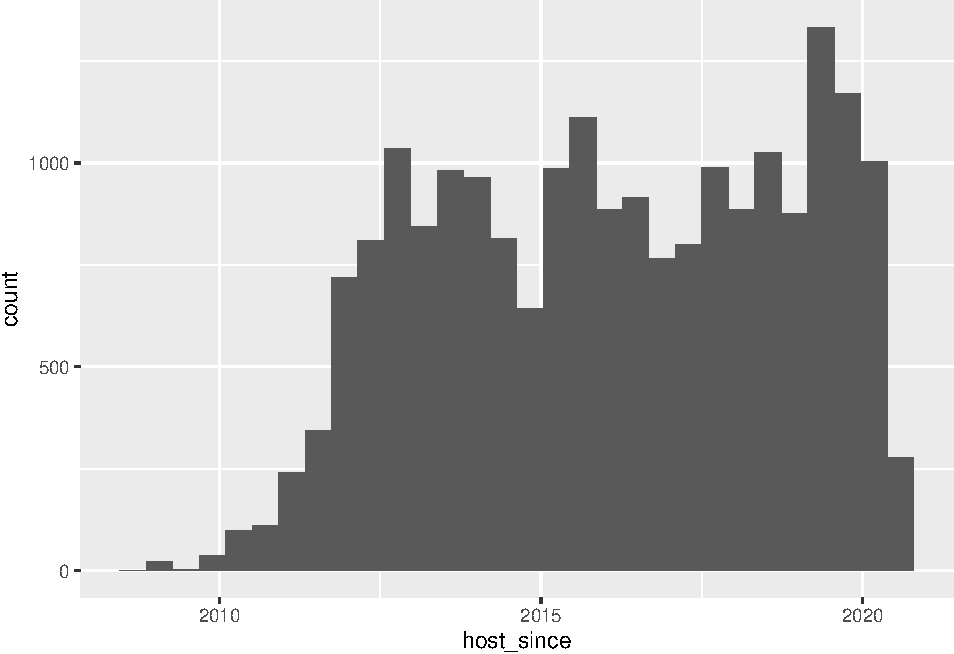
\includegraphics[width=0.5\linewidth]{anal_files/figure-latex/figures-side-1}

\begin{verbatim}
## [1] "variable  15 : host_response_time"
\end{verbatim}

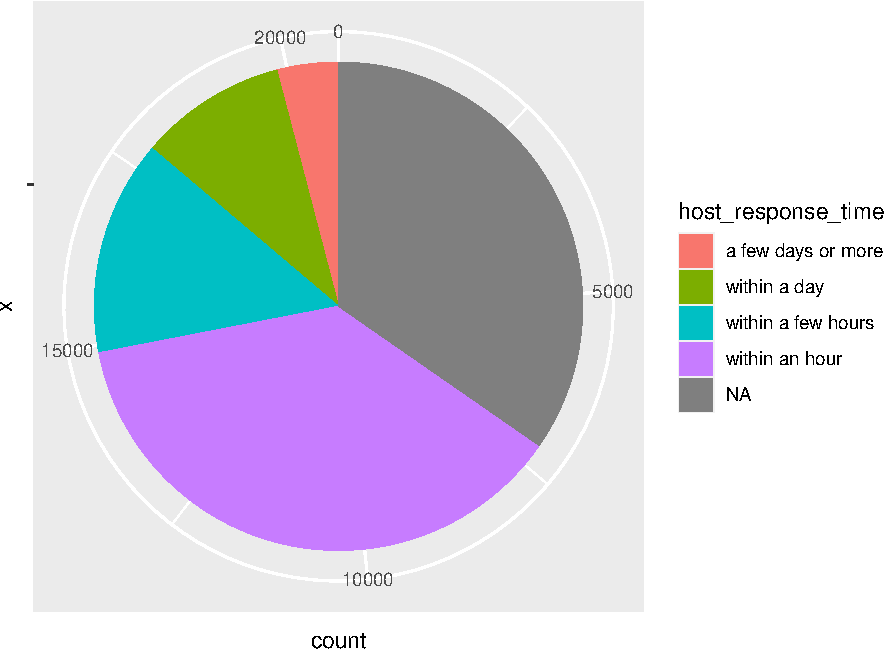
\includegraphics[width=0.5\linewidth]{anal_files/figure-latex/figures-side-2}
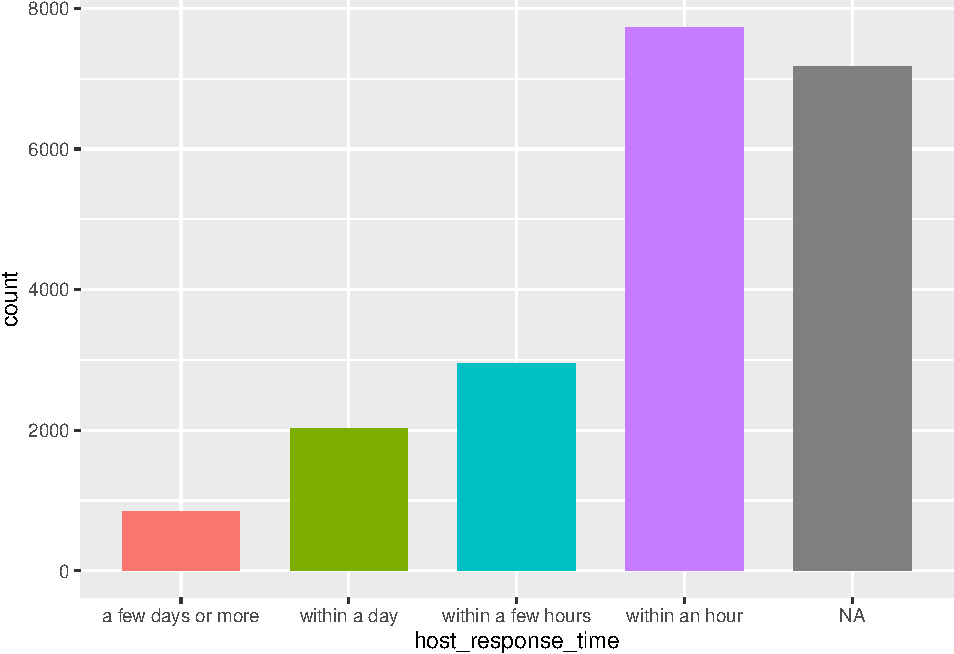
\includegraphics[width=0.5\linewidth]{anal_files/figure-latex/figures-side-3}

\begin{verbatim}
## [1] "Number of modalities:  5"
## [1] "Frequency table"
## 
## a few days or more       within a day within a few hours     within an hour 
##                843               2018               2946               7722 
##               <NA> 
##               7174 
## [1] "Relative frequency table (proportions)"
## 
## a few days or more       within a day within a few hours     within an hour 
##         0.04071874         0.09747380         0.14229822         0.37298942 
##               <NA> 
##         0.34651983 
## [1] "Frequency table sorted"
## 
##     within an hour               <NA> within a few hours       within a day 
##               7722               7174               2946               2018 
## a few days or more 
##                843 
## [1] "Relative frequency table (proportions) sorted"
## 
##     within an hour               <NA> within a few hours       within a day 
##         0.37298942         0.34651983         0.14229822         0.09747380 
## a few days or more 
##         0.04071874 
## [1] "variable  18 : host_is_superhost"
\end{verbatim}

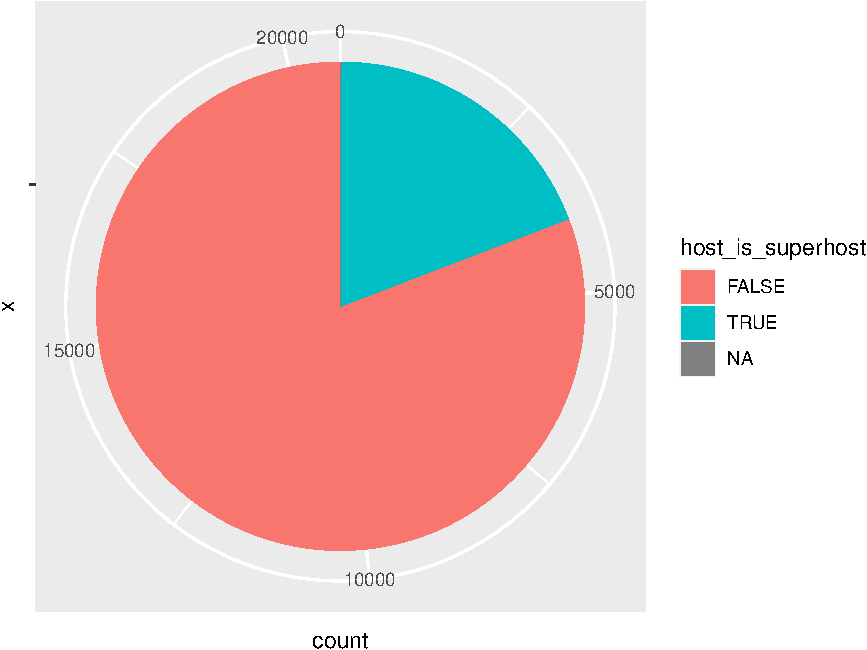
\includegraphics[width=0.5\linewidth]{anal_files/figure-latex/figures-side-4}
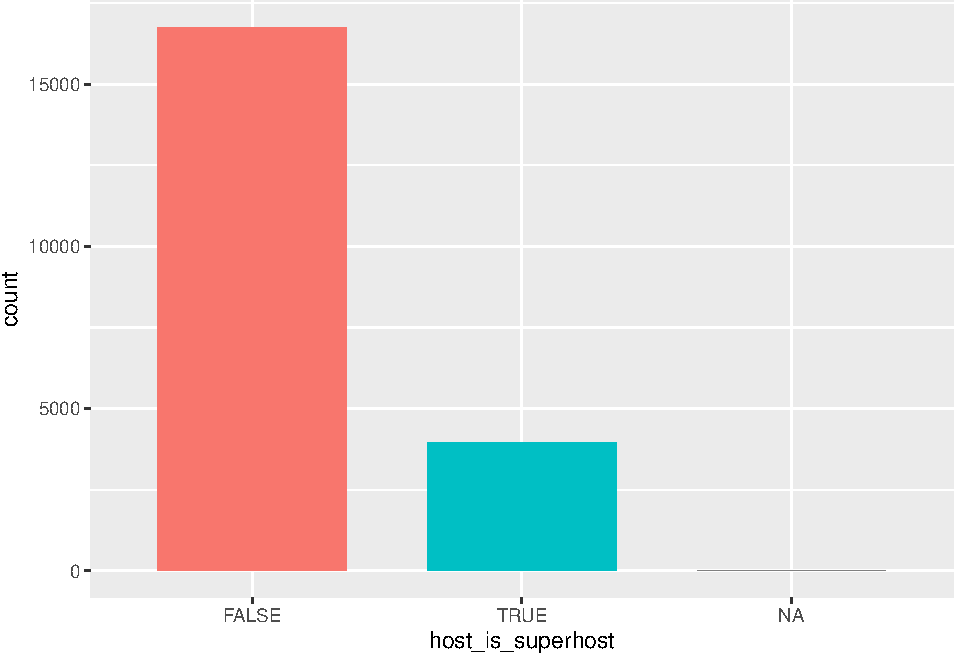
\includegraphics[width=0.5\linewidth]{anal_files/figure-latex/figures-side-5}

\begin{verbatim}
## [1] "Number of modalities:  3"
## [1] "Frequency table"
## 
## FALSE  TRUE  <NA> 
## 16734  3961     8 
## [1] "Relative frequency table (proportions)"
## 
##        FALSE         TRUE         <NA> 
## 0.8082886538 0.1913249288 0.0003864174 
## [1] "Frequency table sorted"
## 
## FALSE  TRUE  <NA> 
## 16734  3961     8 
## [1] "Relative frequency table (proportions) sorted"
## 
##        FALSE         TRUE         <NA> 
## 0.8082886538 0.1913249288 0.0003864174 
## [1] "variable  22 : host_listings_count"
\end{verbatim}

\begin{verbatim}
## `stat_bin()` using `bins = 30`. Pick better value with `binwidth`.
\end{verbatim}

\begin{verbatim}
## Warning: Removed 8 rows containing non-finite values (stat_bin).
\end{verbatim}

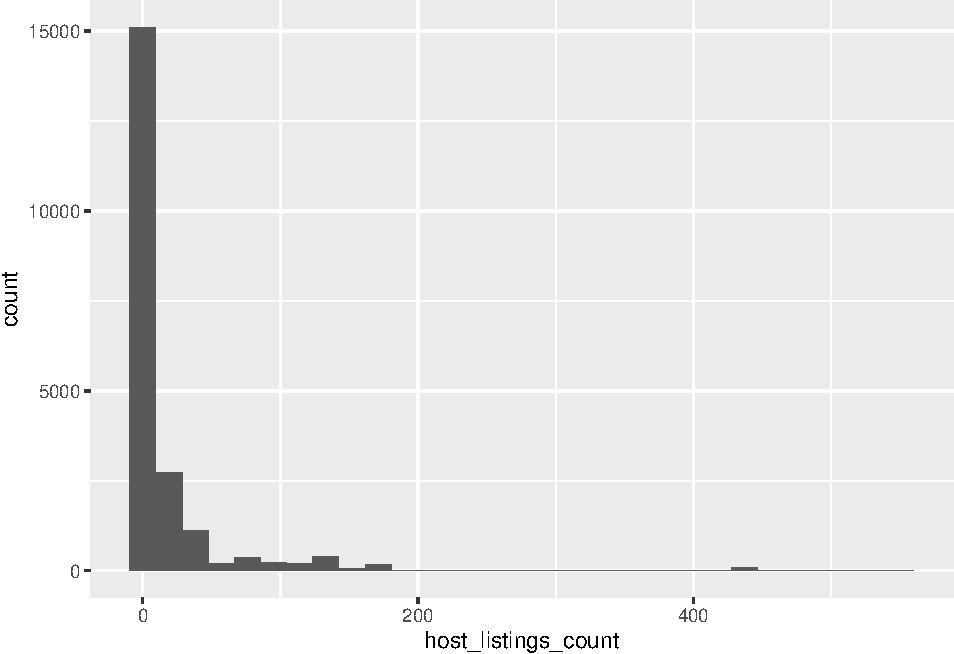
\includegraphics[width=0.5\linewidth]{anal_files/figure-latex/figures-side-6}

\begin{verbatim}
## Warning: Removed 8 rows containing non-finite values (stat_boxplot).
\end{verbatim}

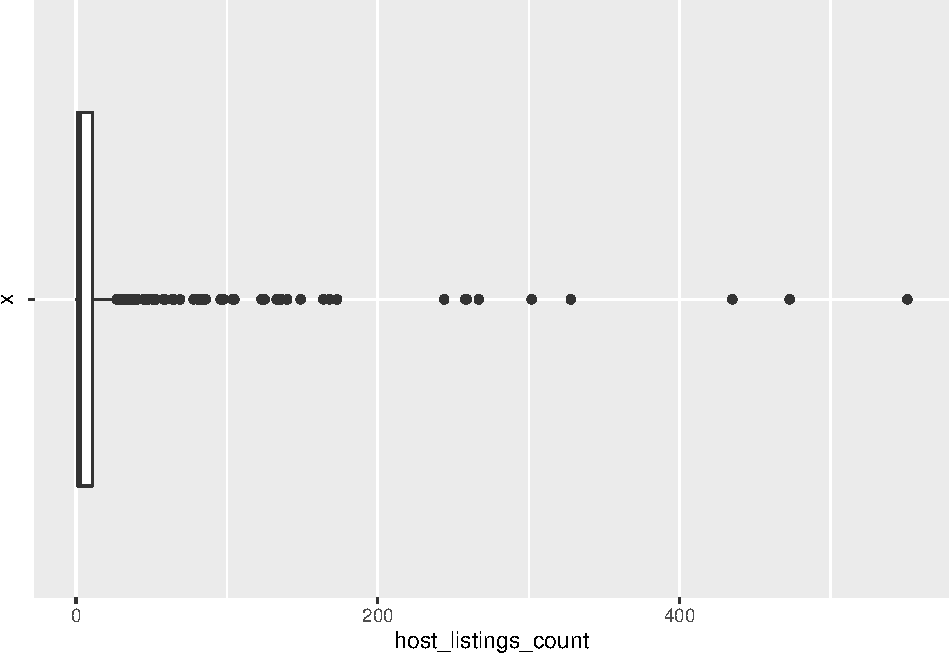
\includegraphics[width=0.5\linewidth]{anal_files/figure-latex/figures-side-7}

\begin{verbatim}
## [1] "Extended Summary Statistics"
##    Min. 1st Qu.  Median    Mean 3rd Qu.    Max.    NA's 
##    0.00    1.00    2.00   16.81   11.00  551.00       8 
## [1] "sd:  43.3787949847988"
## [1] "vc:  2.58000816835102"
## [1] "variable  25 : host_has_profile_pic"
\end{verbatim}

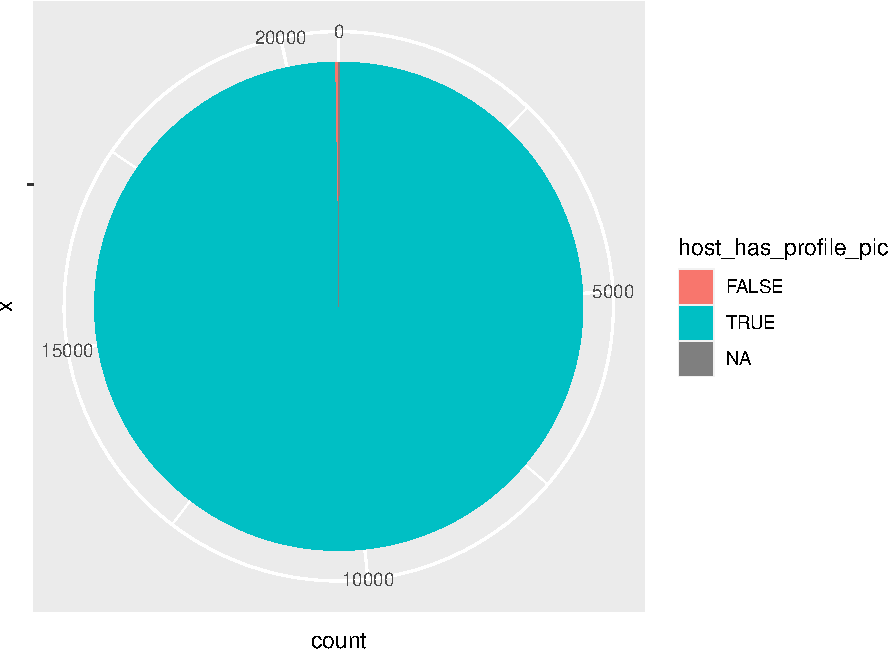
\includegraphics[width=0.5\linewidth]{anal_files/figure-latex/figures-side-8}
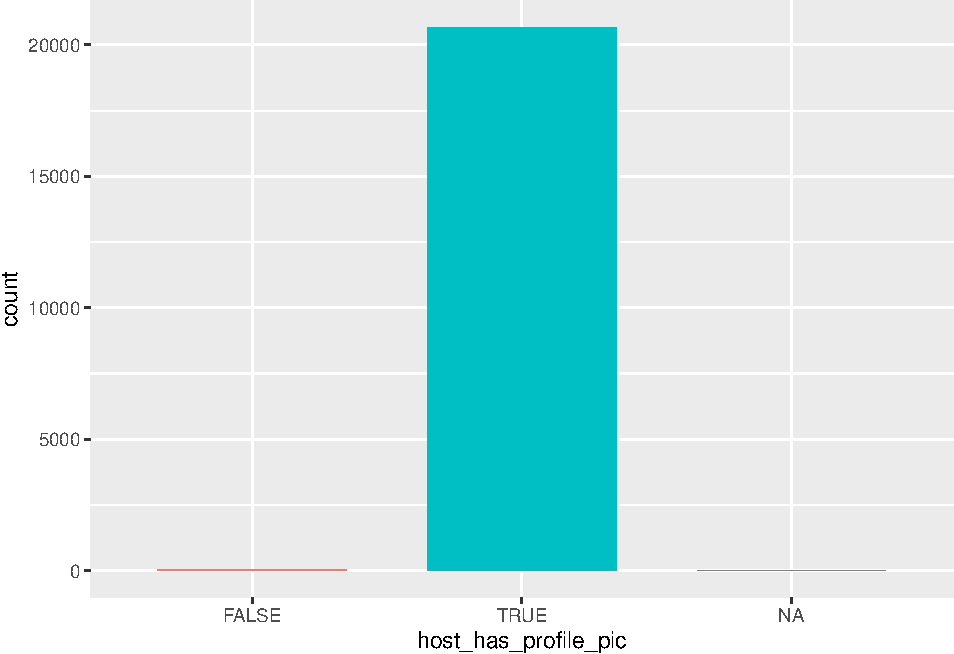
\includegraphics[width=0.5\linewidth]{anal_files/figure-latex/figures-side-9}

\begin{verbatim}
## [1] "Number of modalities:  3"
## [1] "Frequency table"
## 
## FALSE  TRUE  <NA> 
##    55 20640     8 
## [1] "Relative frequency table (proportions)"
## 
##        FALSE         TRUE         <NA> 
## 0.0026566198 0.9969569628 0.0003864174 
## [1] "Frequency table sorted"
## 
##  TRUE FALSE  <NA> 
## 20640    55     8 
## [1] "Relative frequency table (proportions) sorted"
## 
##         TRUE        FALSE         <NA> 
## 0.9969569628 0.0026566198 0.0003864174 
## [1] "variable  26 : host_identity_verified"
\end{verbatim}

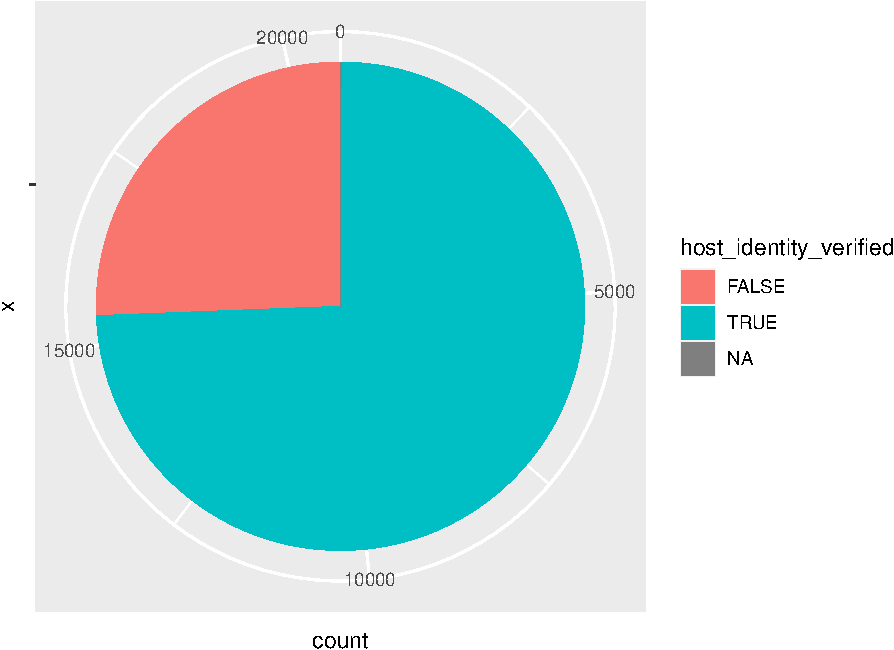
\includegraphics[width=0.5\linewidth]{anal_files/figure-latex/figures-side-10}
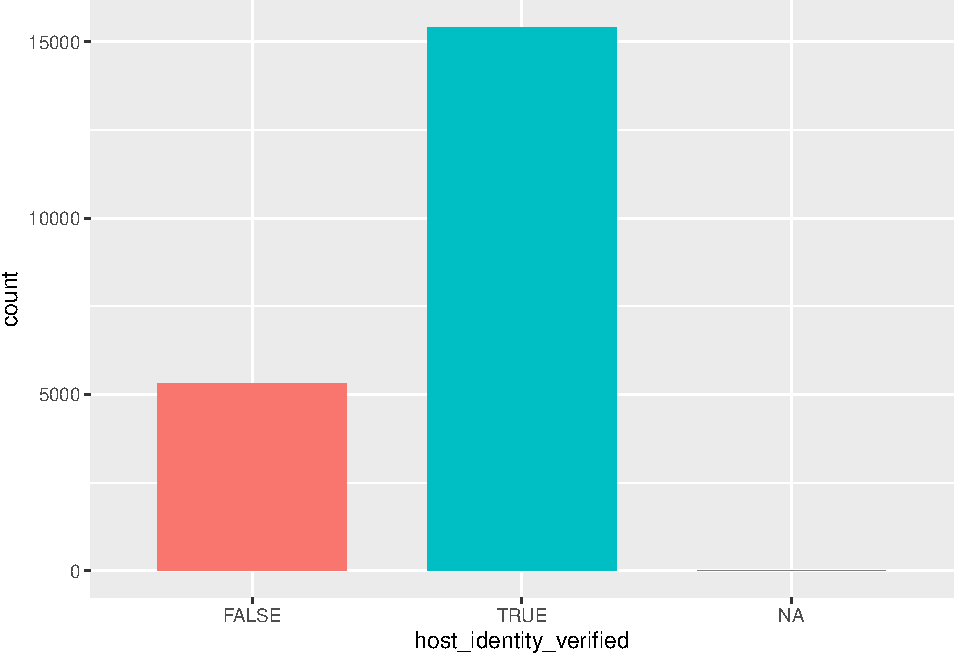
\includegraphics[width=0.5\linewidth]{anal_files/figure-latex/figures-side-11}

\begin{verbatim}
## [1] "Number of modalities:  3"
## [1] "Frequency table"
## 
## FALSE  TRUE  <NA> 
##  5302 15393     8 
## [1] "Relative frequency table (proportions)"
## 
##        FALSE         TRUE         <NA> 
## 0.2560981500 0.7435154325 0.0003864174 
## [1] "Frequency table sorted"
## 
##  TRUE FALSE  <NA> 
## 15393  5302     8 
## [1] "Relative frequency table (proportions) sorted"
## 
##         TRUE        FALSE         <NA> 
## 0.7435154325 0.2560981500 0.0003864174 
## [1] "variable  29 : neighbourhood_group_cleansed"
\end{verbatim}

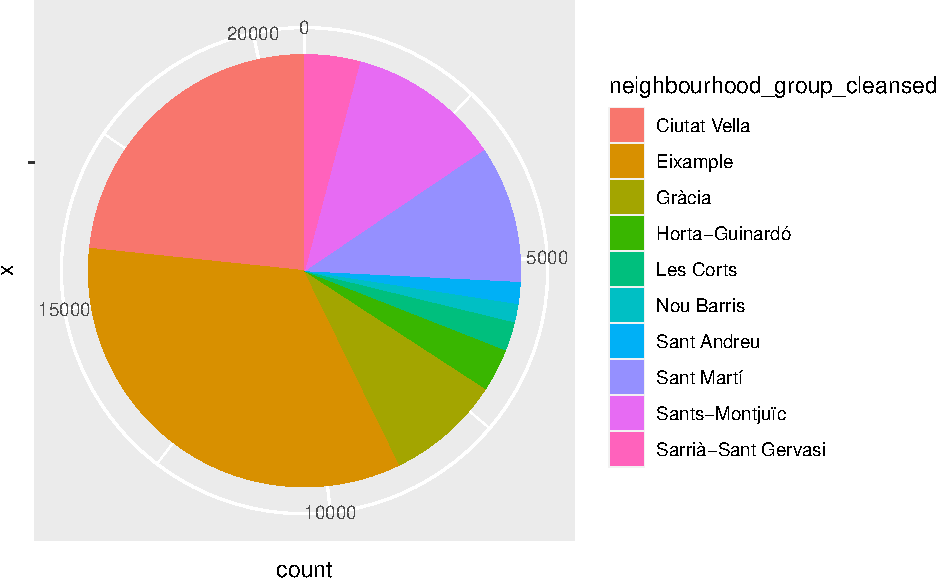
\includegraphics[width=0.5\linewidth]{anal_files/figure-latex/figures-side-12}
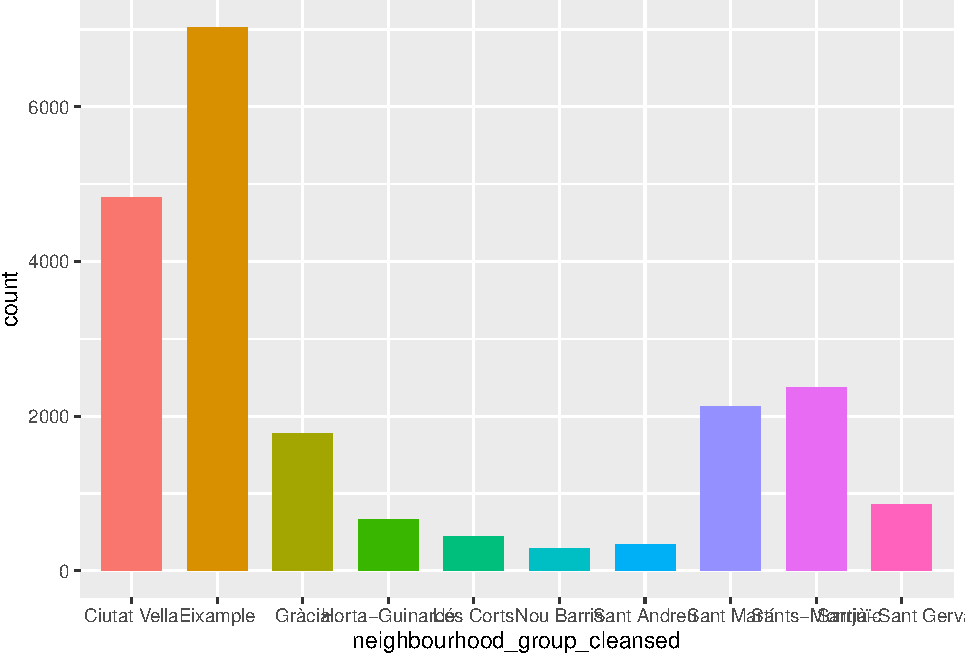
\includegraphics[width=0.5\linewidth]{anal_files/figure-latex/figures-side-13}

\begin{verbatim}
## [1] "Number of modalities:  10"
## [1] "Frequency table"
## 
##        Ciutat Vella            Eixample              Gràcia      Horta-Guinardó 
##                4834                7020                1773                 665 
##           Les Corts          Nou Barris         Sant Andreu          Sant Martí 
##                 448                 284                 339                2123 
##      Sants-Montjuïc Sarrià-Sant Gervasi 
##                2365                 852 
## [1] "Relative frequency table (proportions)"
## 
##        Ciutat Vella            Eixample              Gràcia      Horta-Guinardó 
##          0.23349273          0.33908129          0.08563976          0.03212095 
##           Les Corts          Nou Barris         Sant Andreu          Sant Martí 
##          0.02163938          0.01371782          0.01637444          0.10254552 
##      Sants-Montjuïc Sarrià-Sant Gervasi 
##          0.11423465          0.04115346 
## [1] "Frequency table sorted"
## 
##            Eixample        Ciutat Vella      Sants-Montjuïc          Sant Martí 
##                7020                4834                2365                2123 
##              Gràcia Sarrià-Sant Gervasi      Horta-Guinardó           Les Corts 
##                1773                 852                 665                 448 
##         Sant Andreu          Nou Barris 
##                 339                 284 
## [1] "Relative frequency table (proportions) sorted"
## 
##            Eixample        Ciutat Vella      Sants-Montjuïc          Sant Martí 
##          0.33908129          0.23349273          0.11423465          0.10254552 
##              Gràcia Sarrià-Sant Gervasi      Horta-Guinardó           Les Corts 
##          0.08563976          0.04115346          0.03212095          0.02163938 
##         Sant Andreu          Nou Barris 
##          0.01637444          0.01371782 
## [1] "variable  33 : room_type"
\end{verbatim}

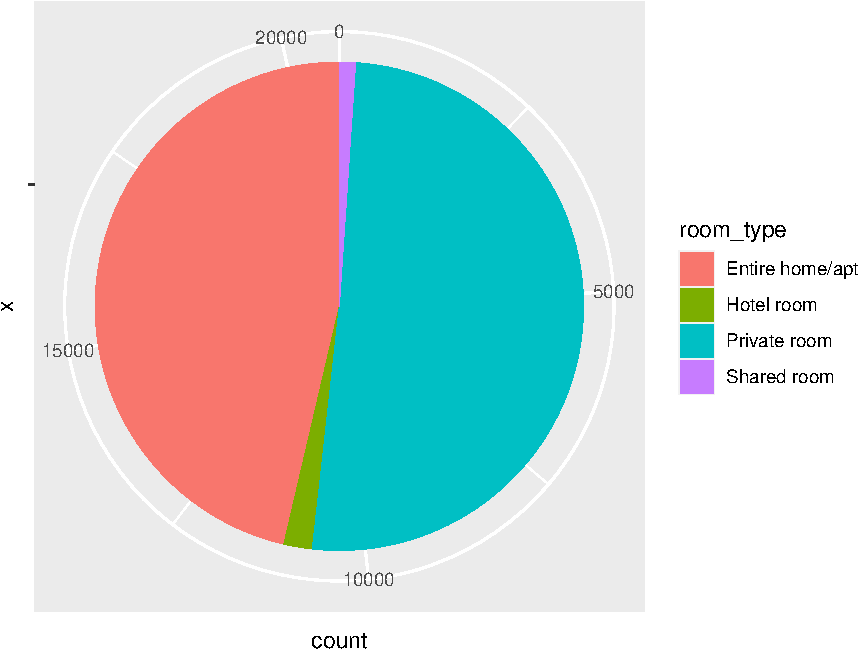
\includegraphics[width=0.5\linewidth]{anal_files/figure-latex/figures-side-14}
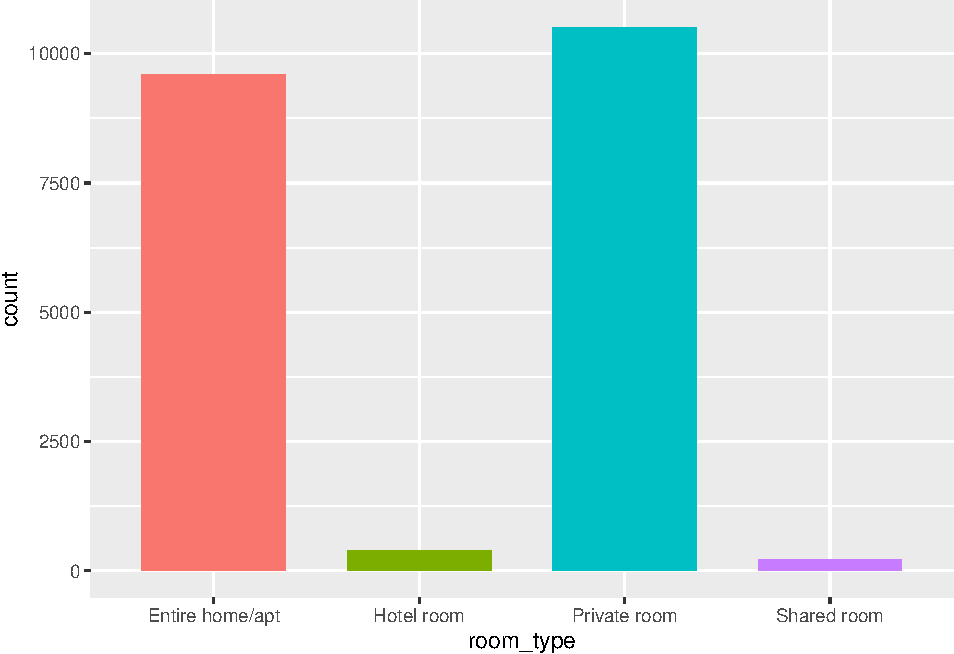
\includegraphics[width=0.5\linewidth]{anal_files/figure-latex/figures-side-15}

\begin{verbatim}
## [1] "Number of modalities:  4"
## [1] "Frequency table"
## 
## Entire home/apt      Hotel room    Private room     Shared room 
##            9596             390           10497             220 
## [1] "Relative frequency table (proportions)"
## 
## Entire home/apt      Hotel room    Private room     Shared room 
##      0.46350770      0.01883785      0.50702797      0.01062648 
## [1] "Frequency table sorted"
## 
##    Private room Entire home/apt      Hotel room     Shared room 
##           10497            9596             390             220 
## [1] "Relative frequency table (proportions) sorted"
## 
##    Private room Entire home/apt      Hotel room     Shared room 
##      0.50702797      0.46350770      0.01883785      0.01062648 
## [1] "variable  34 : accommodates"
\end{verbatim}

\begin{verbatim}
## `stat_bin()` using `bins = 30`. Pick better value with `binwidth`.
\end{verbatim}

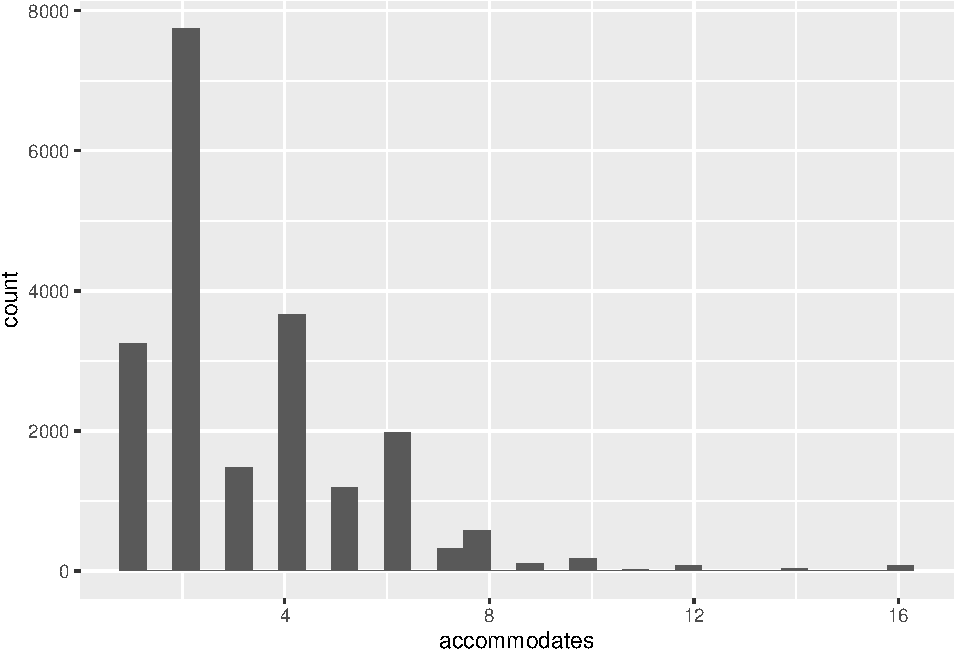
\includegraphics[width=0.5\linewidth]{anal_files/figure-latex/figures-side-16}
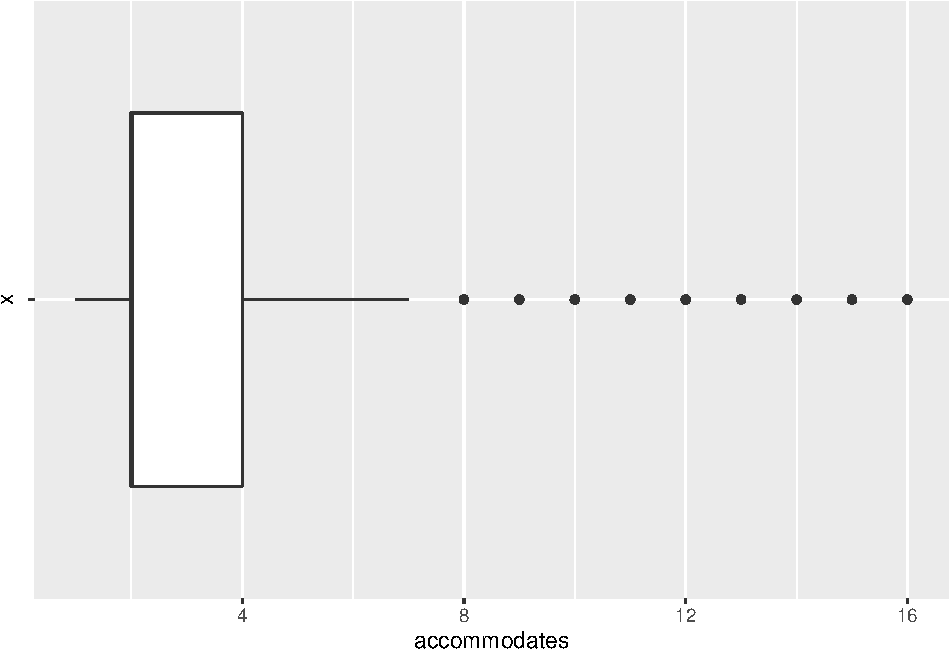
\includegraphics[width=0.5\linewidth]{anal_files/figure-latex/figures-side-17}

\begin{verbatim}
## [1] "Extended Summary Statistics"
##    Min. 1st Qu.  Median    Mean 3rd Qu.    Max. 
##   1.000   2.000   2.000   3.297   4.000  16.000 
## [1] "sd:  2.23873458185074"
## [1] "vc:  0.679109174464914"
## [1] "variable  37 : bedrooms"
\end{verbatim}

\begin{verbatim}
## `stat_bin()` using `bins = 30`. Pick better value with `binwidth`.
\end{verbatim}

\begin{verbatim}
## Warning: Removed 684 rows containing non-finite values (stat_bin).
\end{verbatim}

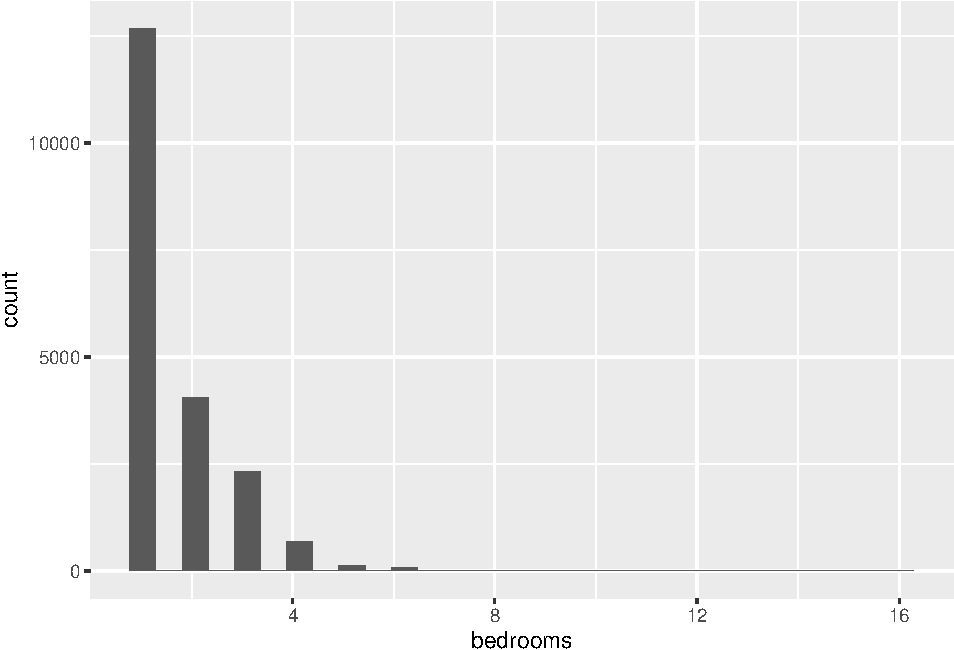
\includegraphics[width=0.5\linewidth]{anal_files/figure-latex/figures-side-18}

\begin{verbatim}
## Warning: Removed 684 rows containing non-finite values (stat_boxplot).
\end{verbatim}

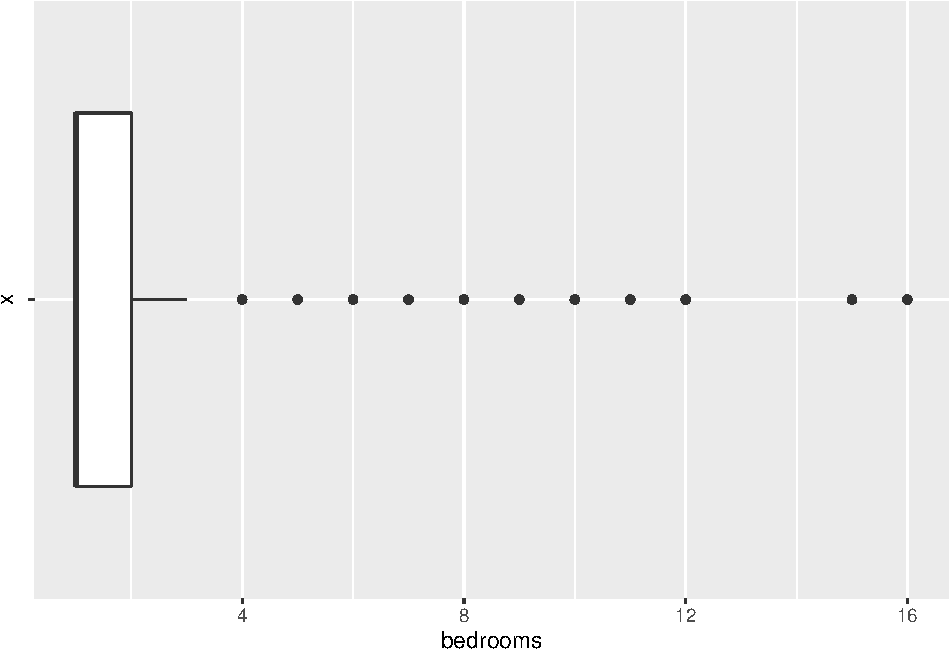
\includegraphics[width=0.5\linewidth]{anal_files/figure-latex/figures-side-19}

\begin{verbatim}
## [1] "Extended Summary Statistics"
##    Min. 1st Qu.  Median    Mean 3rd Qu.    Max.    NA's 
##   1.000   1.000   1.000   1.604   2.000  16.000     684 
## [1] "sd:  0.991927540847893"
## [1] "vc:  0.618398599864033"
## [1] "variable  38 : beds"
\end{verbatim}

\begin{verbatim}
## `stat_bin()` using `bins = 30`. Pick better value with `binwidth`.
\end{verbatim}

\begin{verbatim}
## Warning: Removed 409 rows containing non-finite values (stat_bin).
\end{verbatim}

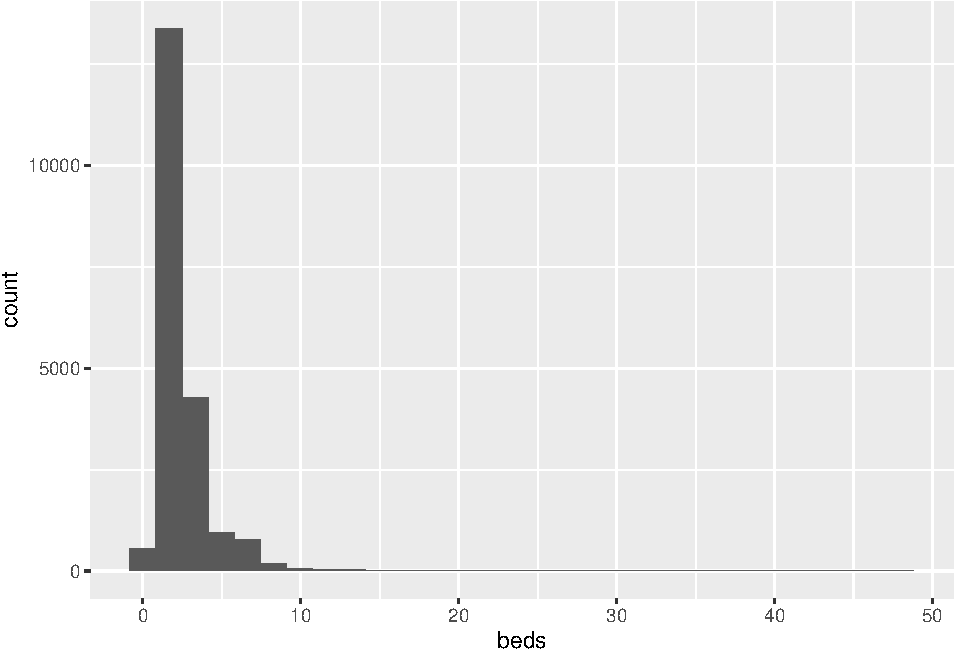
\includegraphics[width=0.5\linewidth]{anal_files/figure-latex/figures-side-20}

\begin{verbatim}
## Warning: Removed 409 rows containing non-finite values (stat_boxplot).
\end{verbatim}

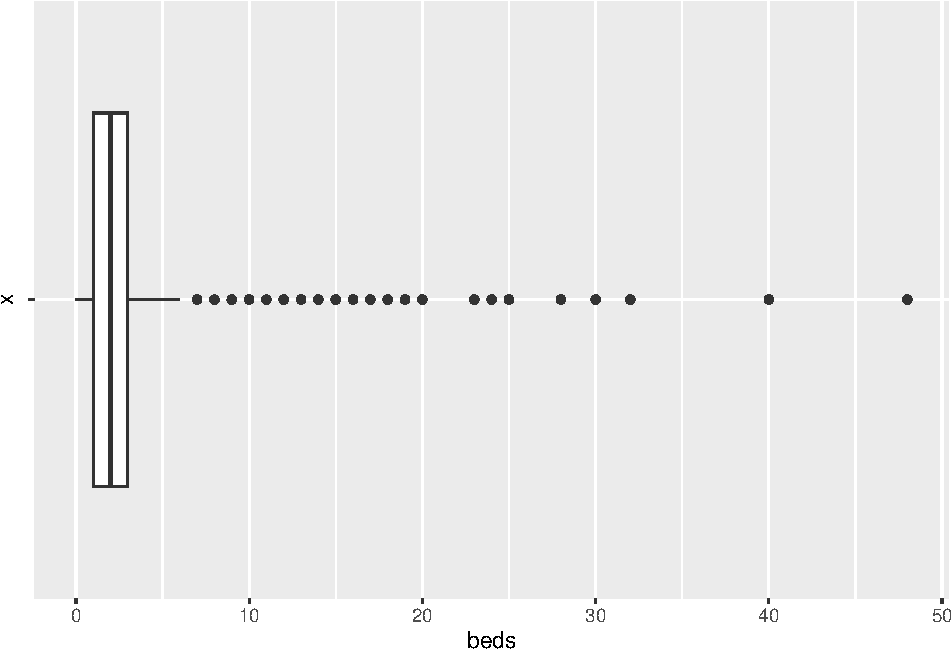
\includegraphics[width=0.5\linewidth]{anal_files/figure-latex/figures-side-21}

\begin{verbatim}
## [1] "Extended Summary Statistics"
##    Min. 1st Qu.  Median    Mean 3rd Qu.    Max.    NA's 
##   0.000   1.000   2.000   2.233   3.000  48.000     409 
## [1] "sd:  1.9777846692546"
## [1] "vc:  0.885854070446331"
## [1] "variable  40 : price"
\end{verbatim}

\begin{verbatim}
## `stat_bin()` using `bins = 30`. Pick better value with `binwidth`.
\end{verbatim}

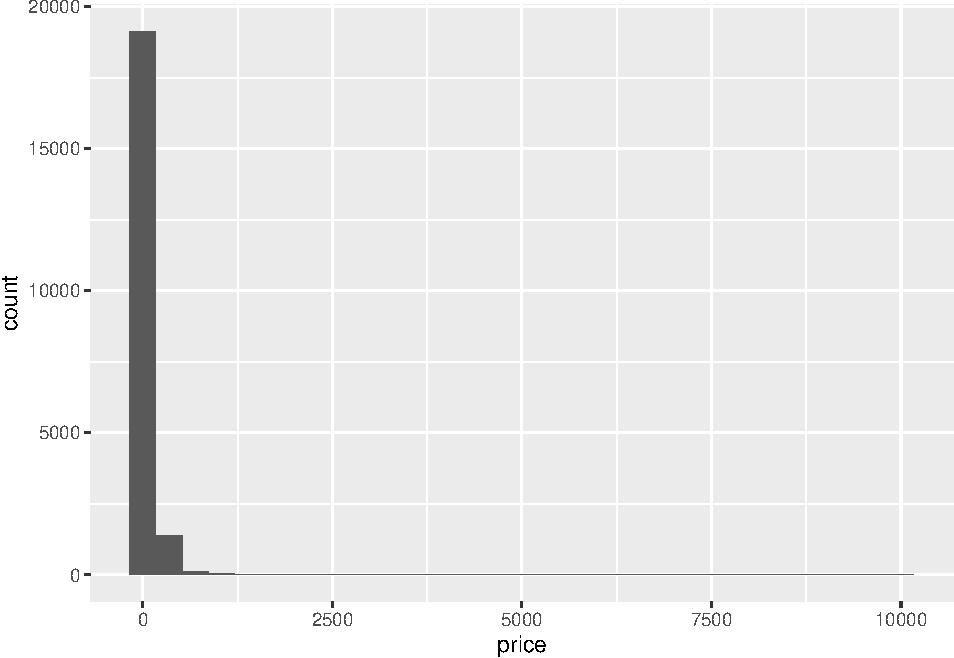
\includegraphics[width=0.5\linewidth]{anal_files/figure-latex/figures-side-22}
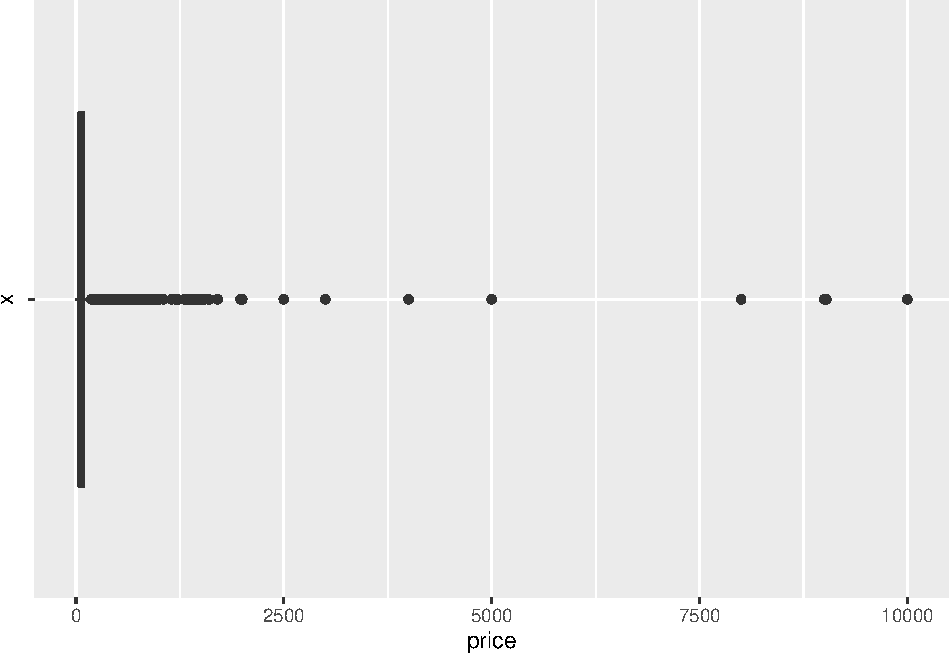
\includegraphics[width=0.5\linewidth]{anal_files/figure-latex/figures-side-23}

\begin{verbatim}
## [1] "Extended Summary Statistics"
##     Min.  1st Qu.   Median     Mean  3rd Qu.     Max. 
##     0.00    35.00    55.00    86.34    95.00 10000.00 
## [1] "sd:  206.462373757297"
## [1] "vc:  2.39112430629807"
## [1] "variable  47 : minimum_nights_avg_ntm"
\end{verbatim}

\begin{verbatim}
## `stat_bin()` using `bins = 30`. Pick better value with `binwidth`.
\end{verbatim}

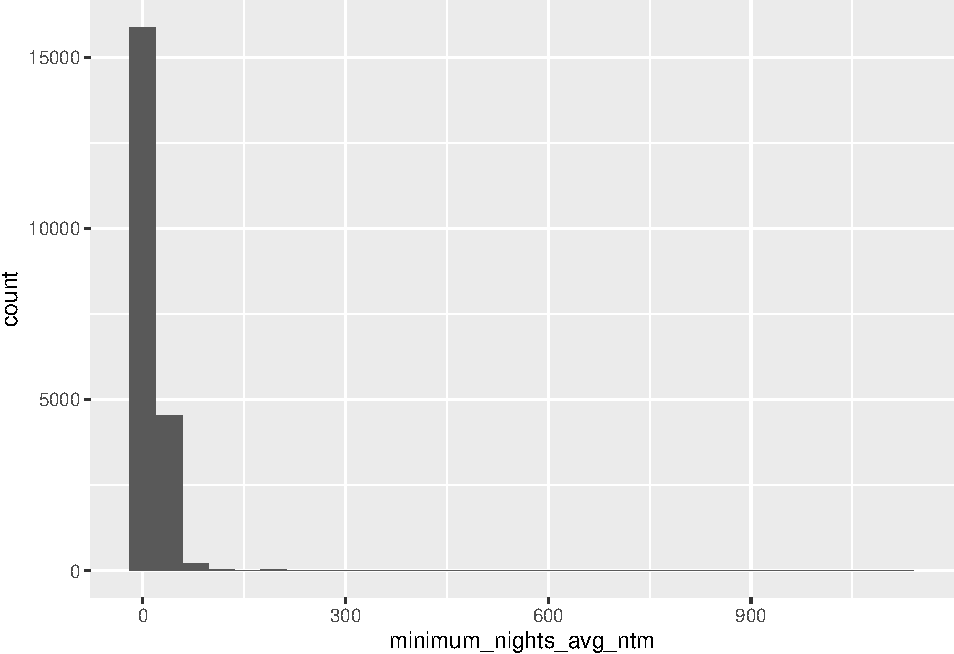
\includegraphics[width=0.5\linewidth]{anal_files/figure-latex/figures-side-24}
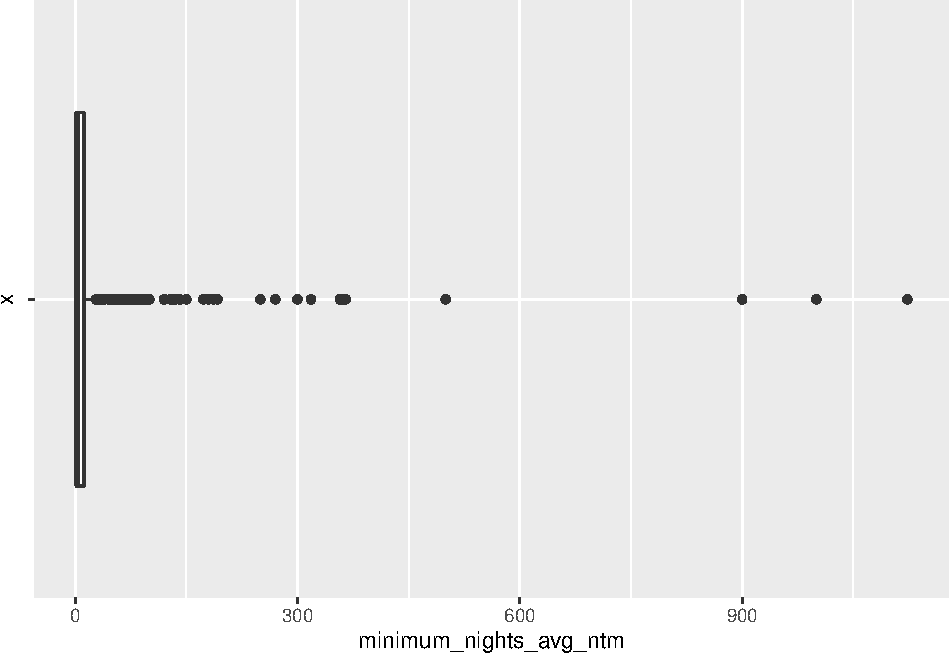
\includegraphics[width=0.5\linewidth]{anal_files/figure-latex/figures-side-25}

\begin{verbatim}
## [1] "Extended Summary Statistics"
##    Min. 1st Qu.  Median    Mean 3rd Qu.    Max. 
##    1.00    1.40    2.70   10.67   12.10 1123.00 
## [1] "sd:  25.7663823069"
## [1] "vc:  2.41544083534869"
## [1] "variable  48 : maximum_nights_avg_ntm"
\end{verbatim}

\begin{verbatim}
## `stat_bin()` using `bins = 30`. Pick better value with `binwidth`.
\end{verbatim}

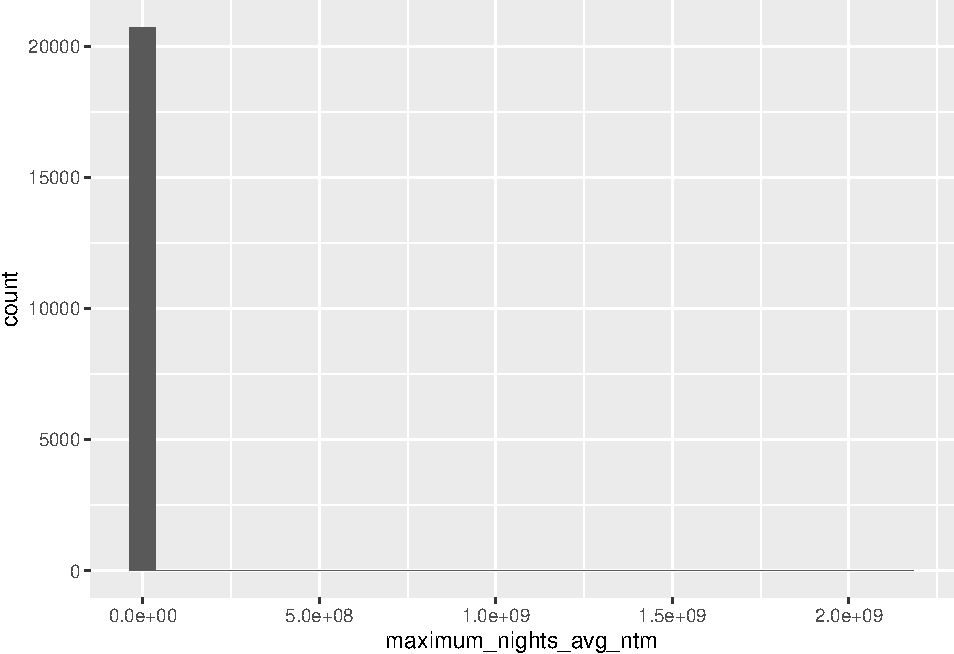
\includegraphics[width=0.5\linewidth]{anal_files/figure-latex/figures-side-26}
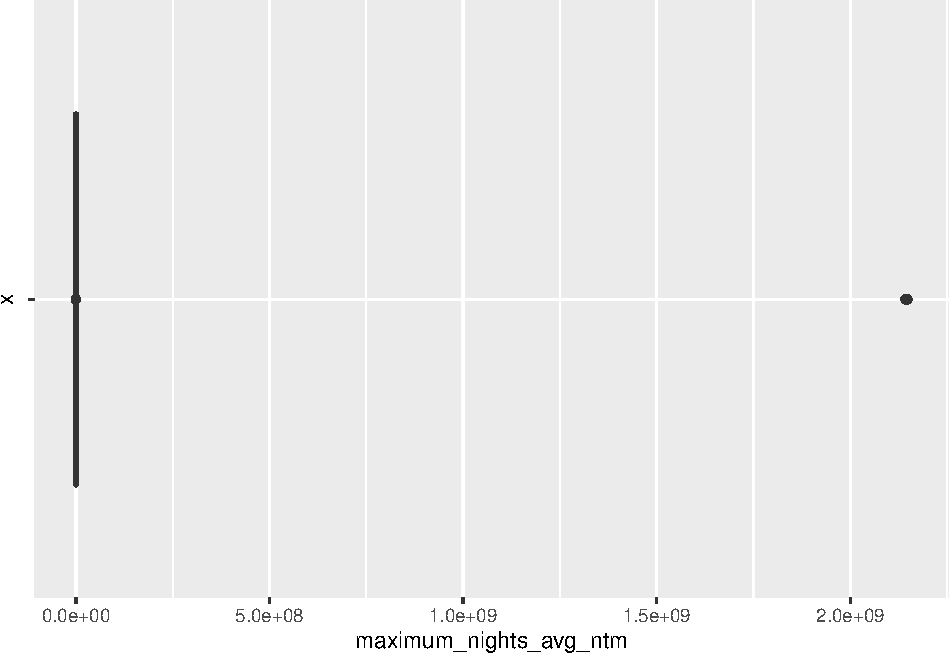
\includegraphics[width=0.5\linewidth]{anal_files/figure-latex/figures-side-27}

\begin{verbatim}
## [1] "Extended Summary Statistics"
##      Min.   1st Qu.    Median      Mean   3rd Qu.      Max. 
## 1.000e+00 3.300e+02 1.125e+03 3.118e+05 1.125e+03 2.147e+09 
## [1] "sd:  25829740.5605248"
## [1] "vc:  82.8528295497124"
## [1] "variable  51 : availability_30"
\end{verbatim}

\begin{verbatim}
## `stat_bin()` using `bins = 30`. Pick better value with `binwidth`.
\end{verbatim}

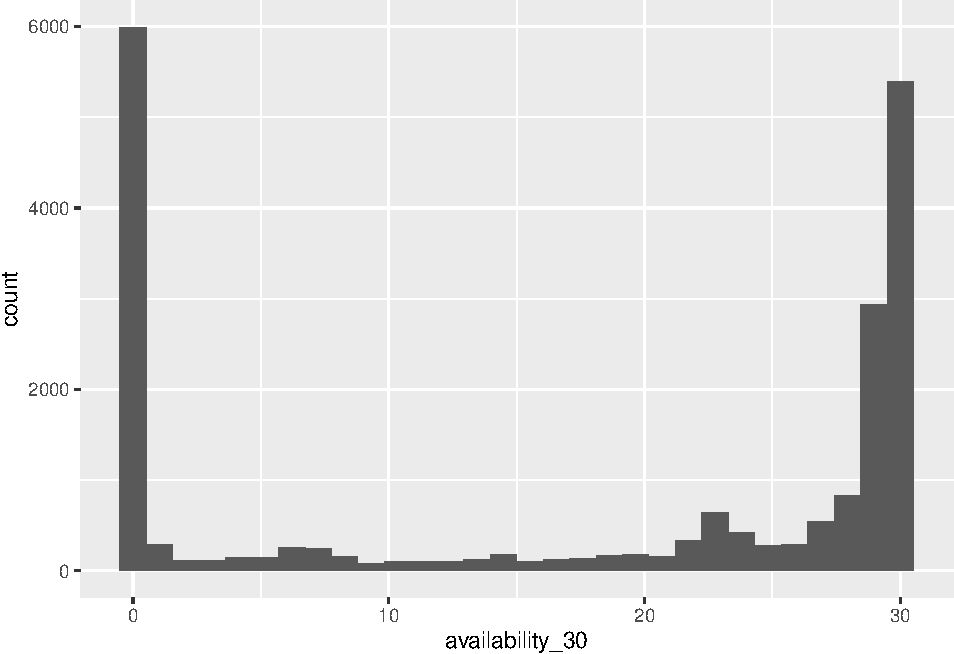
\includegraphics[width=0.5\linewidth]{anal_files/figure-latex/figures-side-28}
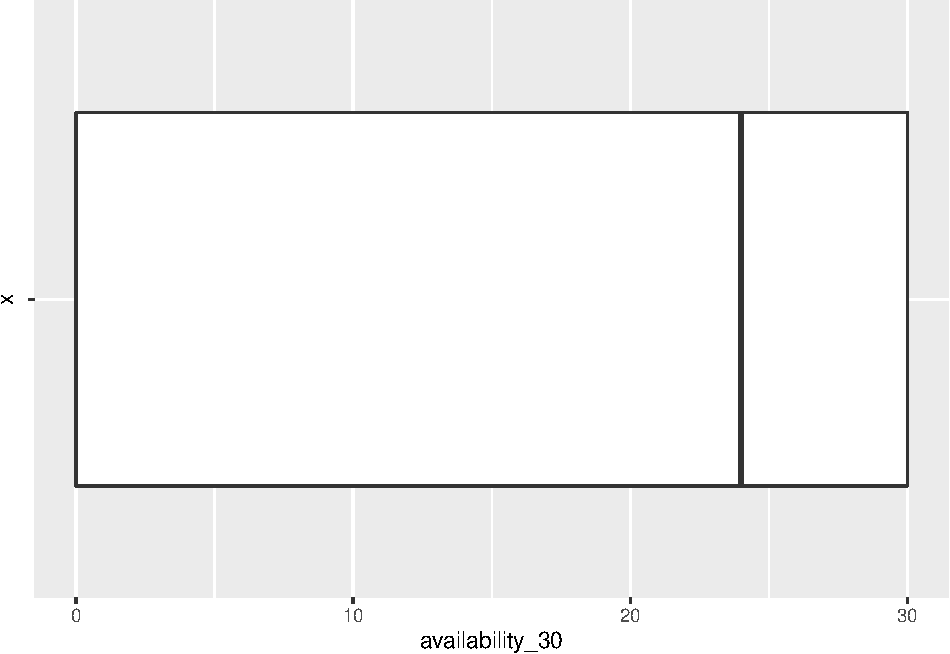
\includegraphics[width=0.5\linewidth]{anal_files/figure-latex/figures-side-29}

\begin{verbatim}
## [1] "Extended Summary Statistics"
##    Min. 1st Qu.  Median    Mean 3rd Qu.    Max. 
##    0.00    0.00   24.00   17.55   30.00   30.00 
## [1] "sd:  13.1256857815973"
## [1] "vc:  0.748066313023828"
## [1] "variable  52 : availability_60"
\end{verbatim}

\begin{verbatim}
## `stat_bin()` using `bins = 30`. Pick better value with `binwidth`.
\end{verbatim}

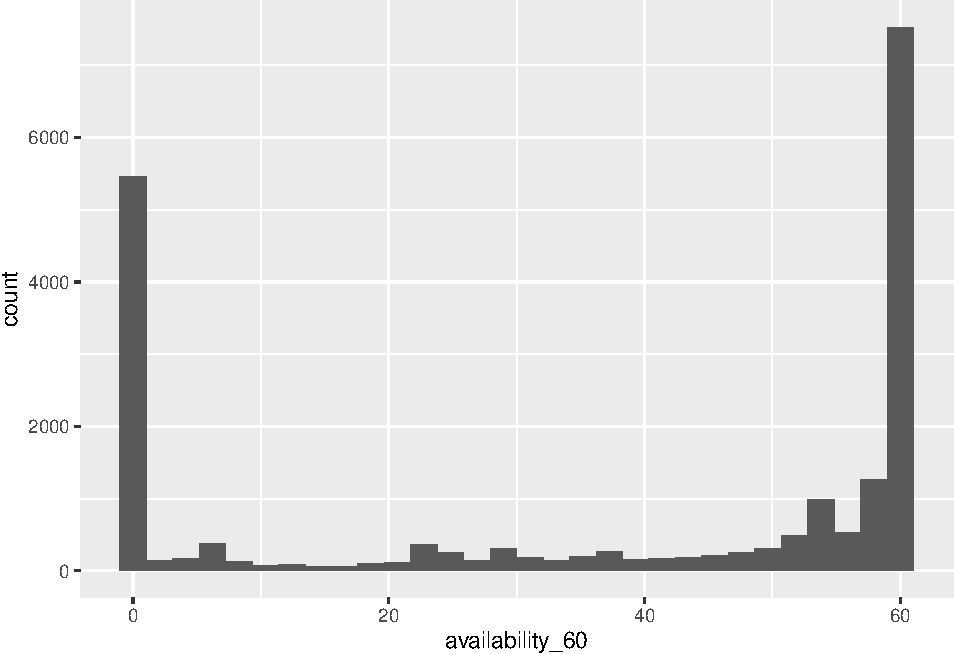
\includegraphics[width=0.5\linewidth]{anal_files/figure-latex/figures-side-30}
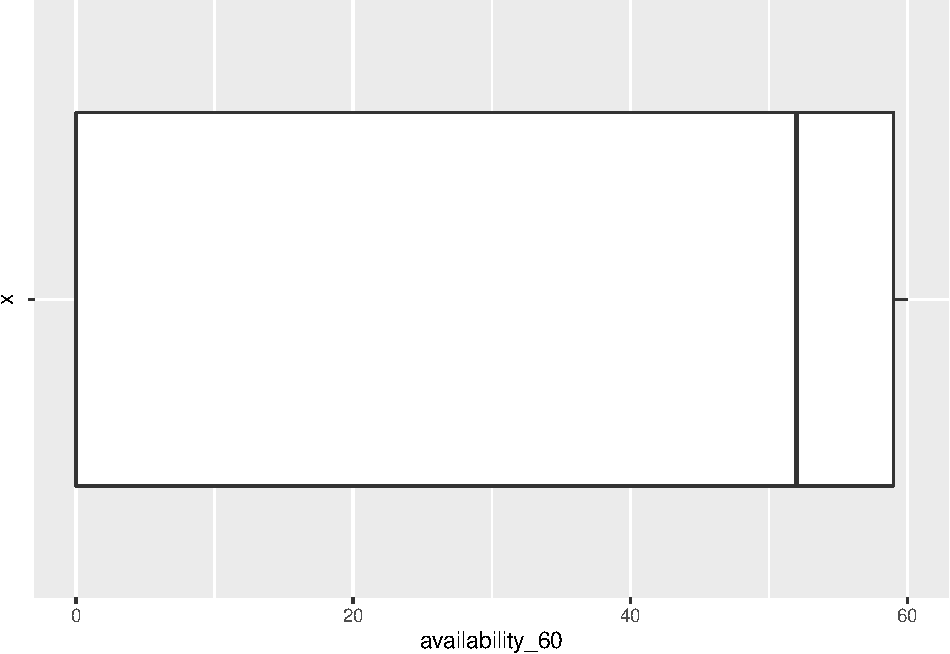
\includegraphics[width=0.5\linewidth]{anal_files/figure-latex/figures-side-31}

\begin{verbatim}
## [1] "Extended Summary Statistics"
##    Min. 1st Qu.  Median    Mean 3rd Qu.    Max. 
##    0.00    0.00   52.00   36.43   59.00   60.00 
## [1] "sd:  25.7246770560561"
## [1] "vc:  0.706174828708438"
## [1] "variable  53 : availability_90"
\end{verbatim}

\begin{verbatim}
## `stat_bin()` using `bins = 30`. Pick better value with `binwidth`.
\end{verbatim}

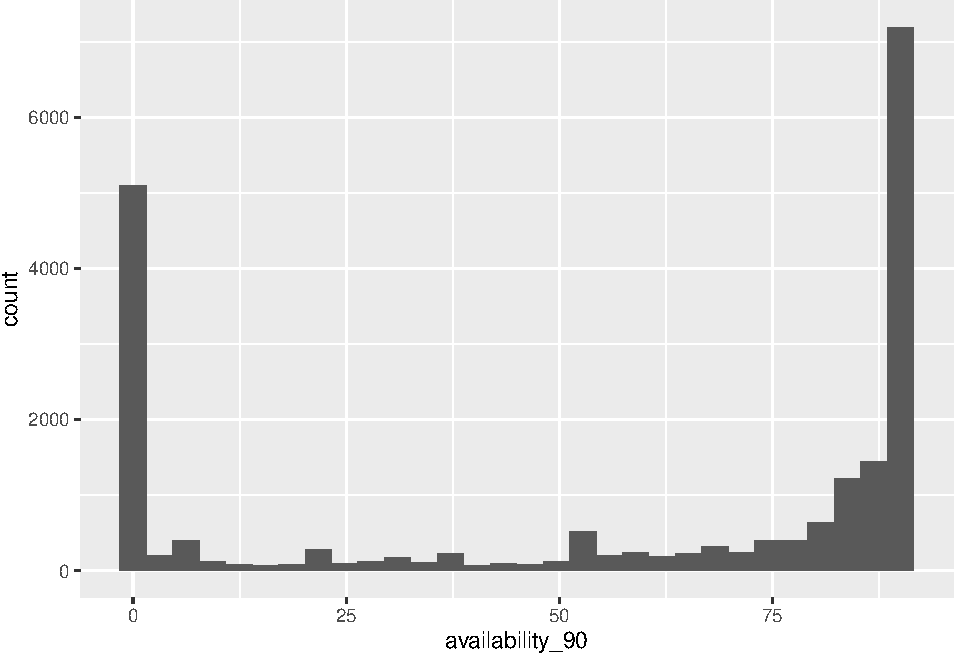
\includegraphics[width=0.5\linewidth]{anal_files/figure-latex/figures-side-32}
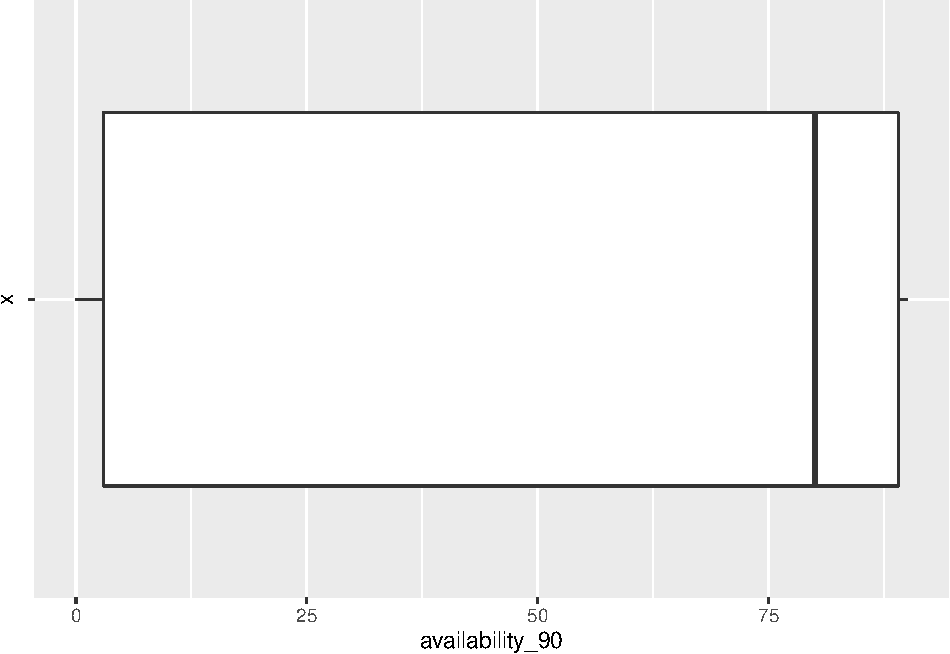
\includegraphics[width=0.5\linewidth]{anal_files/figure-latex/figures-side-33}

\begin{verbatim}
## [1] "Extended Summary Statistics"
##    Min. 1st Qu.  Median    Mean 3rd Qu.    Max. 
##    0.00    3.00   80.00   56.01   89.00   90.00 
## [1] "sd:  38.3144345211077"
## [1] "vc:  0.684065373969981"
## [1] "variable  54 : availability_365"
\end{verbatim}

\begin{verbatim}
## `stat_bin()` using `bins = 30`. Pick better value with `binwidth`.
\end{verbatim}

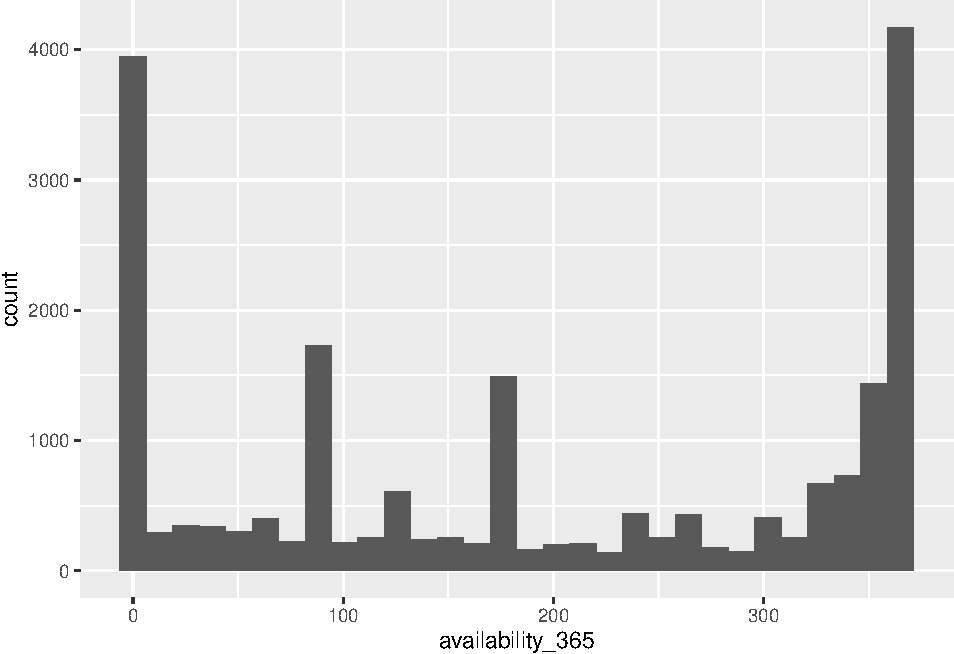
\includegraphics[width=0.5\linewidth]{anal_files/figure-latex/figures-side-34}
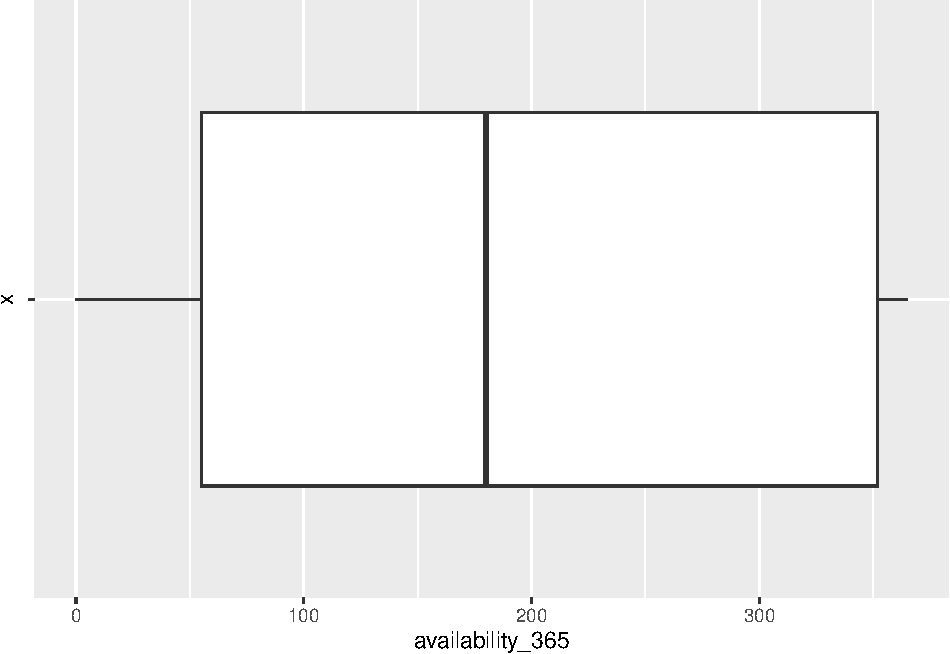
\includegraphics[width=0.5\linewidth]{anal_files/figure-latex/figures-side-35}

\begin{verbatim}
## [1] "Extended Summary Statistics"
##    Min. 1st Qu.  Median    Mean 3rd Qu.    Max. 
##     0.0    55.0   180.0   191.3   352.0   365.0 
## [1] "sd:  142.34942312352"
## [1] "vc:  0.744162184889913"
## [1] "variable  56 : number_of_reviews"
\end{verbatim}

\begin{verbatim}
## `stat_bin()` using `bins = 30`. Pick better value with `binwidth`.
\end{verbatim}

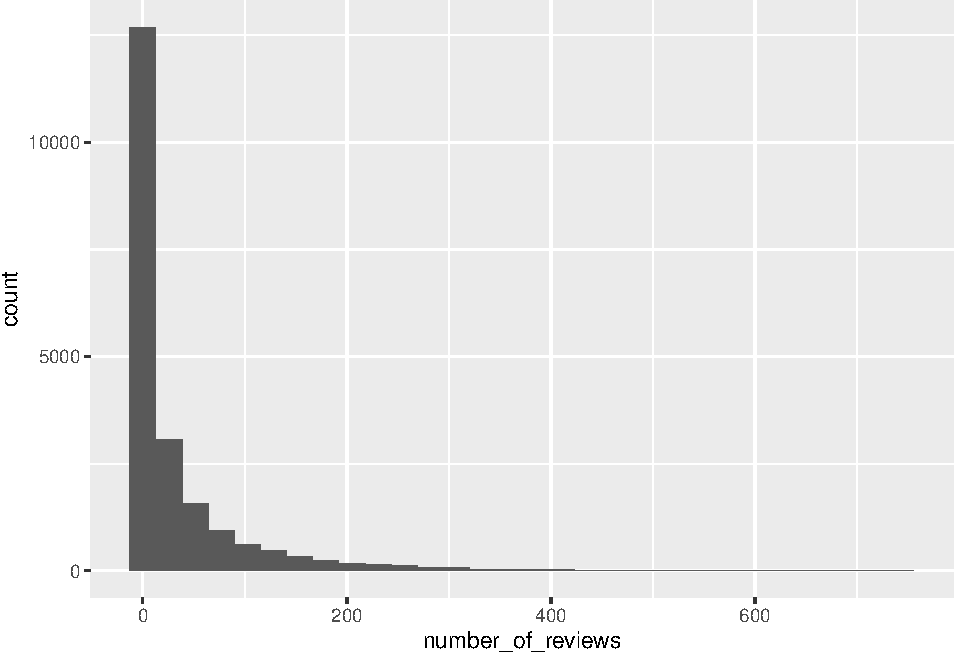
\includegraphics[width=0.5\linewidth]{anal_files/figure-latex/figures-side-36}
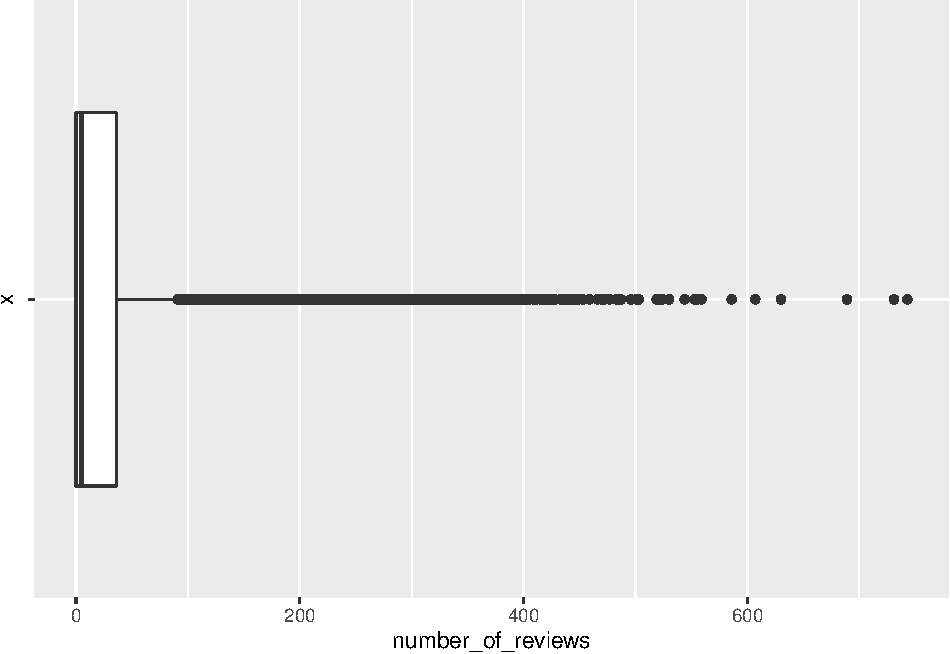
\includegraphics[width=0.5\linewidth]{anal_files/figure-latex/figures-side-37}

\begin{verbatim}
## [1] "Extended Summary Statistics"
##    Min. 1st Qu.  Median    Mean 3rd Qu.    Max. 
##     0.0     0.0     5.0    33.1    36.0   743.0 
## [1] "sd:  63.3189933063887"
## [1] "vc:  1.91281341970952"
## [1] "variable  57 : number_of_reviews_ltm"
\end{verbatim}

\begin{verbatim}
## `stat_bin()` using `bins = 30`. Pick better value with `binwidth`.
\end{verbatim}

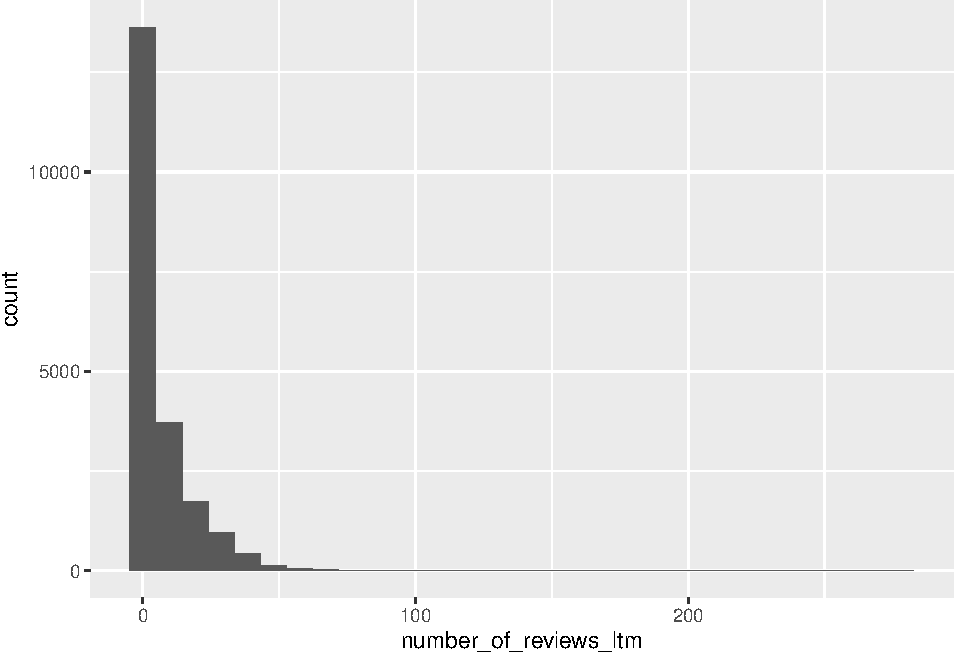
\includegraphics[width=0.5\linewidth]{anal_files/figure-latex/figures-side-38}
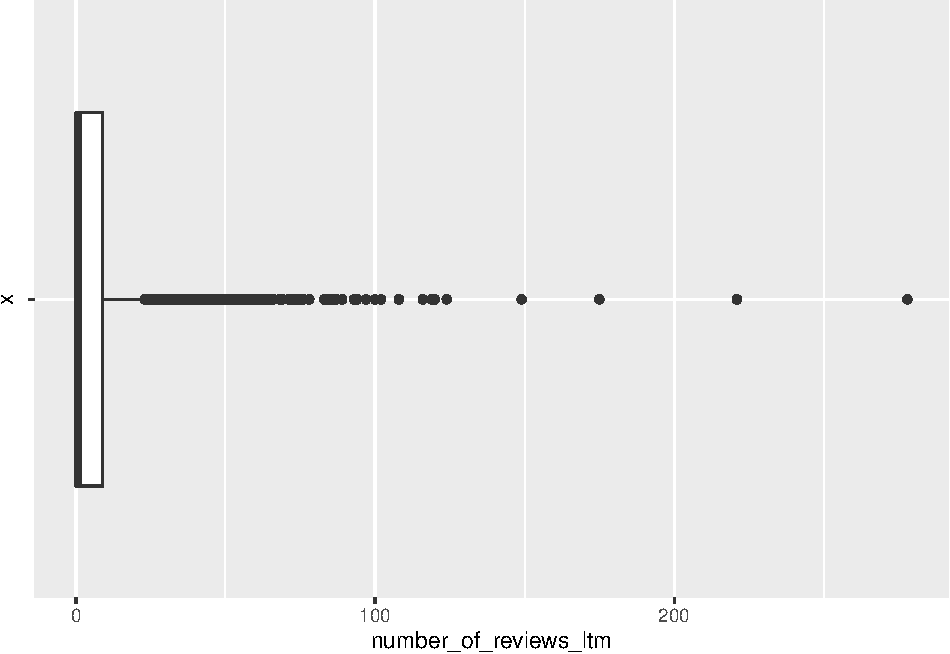
\includegraphics[width=0.5\linewidth]{anal_files/figure-latex/figures-side-39}

\begin{verbatim}
## [1] "Extended Summary Statistics"
##    Min. 1st Qu.  Median    Mean 3rd Qu.    Max. 
##   0.000   0.000   1.000   6.401   9.000 278.000 
## [1] "sd:  11.1280843101846"
## [1] "vc:  1.73849026164919"
## [1] "variable  58 : number_of_reviews_l30d"
\end{verbatim}

\begin{verbatim}
## `stat_bin()` using `bins = 30`. Pick better value with `binwidth`.
\end{verbatim}

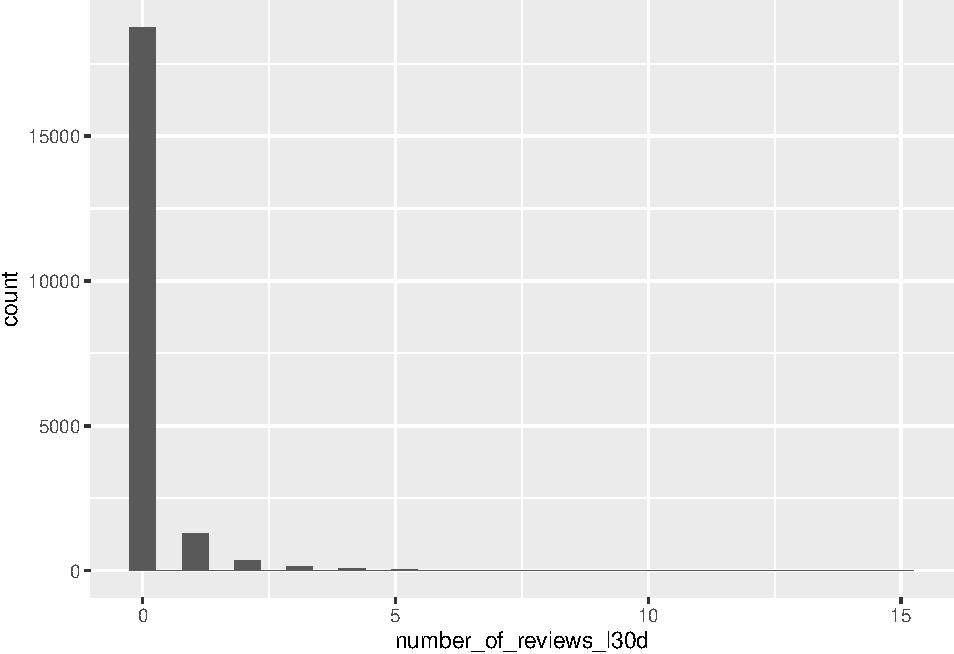
\includegraphics[width=0.5\linewidth]{anal_files/figure-latex/figures-side-40}
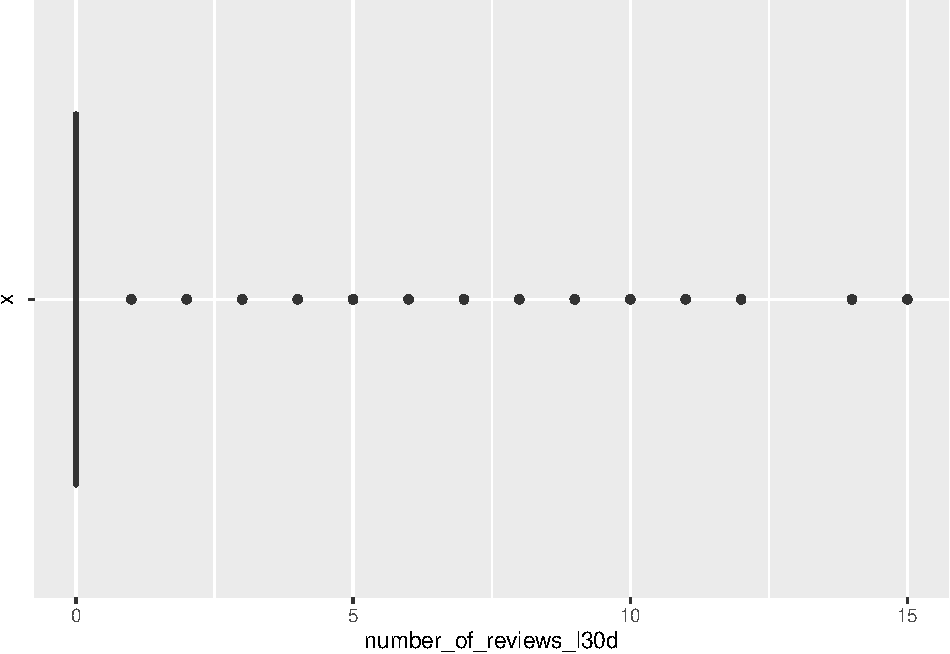
\includegraphics[width=0.5\linewidth]{anal_files/figure-latex/figures-side-41}

\begin{verbatim}
## [1] "Extended Summary Statistics"
##    Min. 1st Qu.  Median    Mean 3rd Qu.    Max. 
##  0.0000  0.0000  0.0000  0.1621  0.0000 15.0000 
## [1] "sd:  0.661615277330759"
## [1] "vc:  4.0814723142368"
## [1] "variable  61 : review_scores_rating"
\end{verbatim}

\begin{verbatim}
## `stat_bin()` using `bins = 30`. Pick better value with `binwidth`.
\end{verbatim}

\begin{verbatim}
## Warning: Removed 5971 rows containing non-finite values (stat_bin).
\end{verbatim}

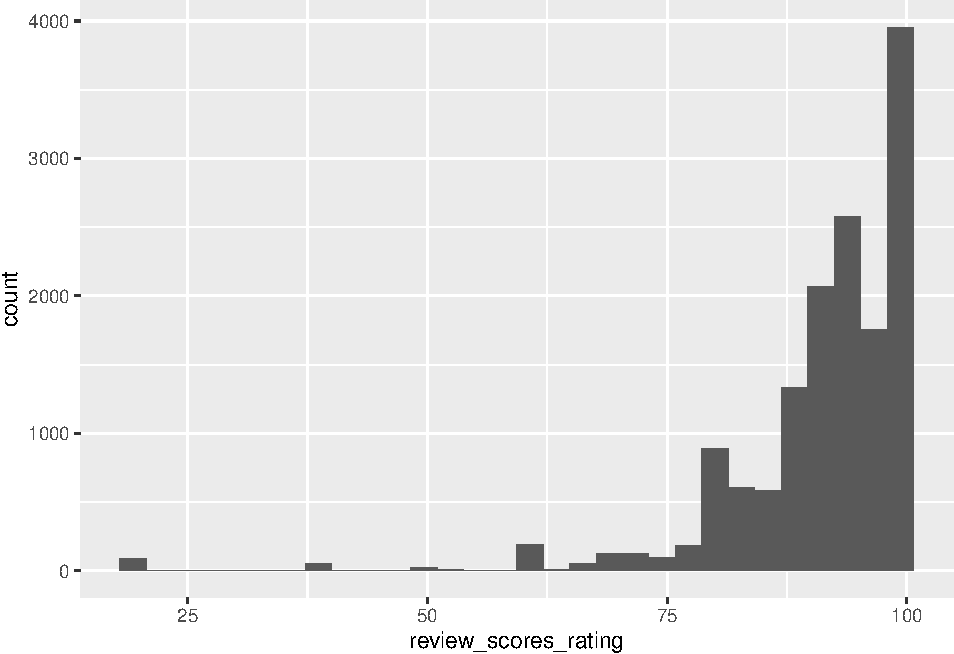
\includegraphics[width=0.5\linewidth]{anal_files/figure-latex/figures-side-42}

\begin{verbatim}
## Warning: Removed 5971 rows containing non-finite values (stat_boxplot).
\end{verbatim}

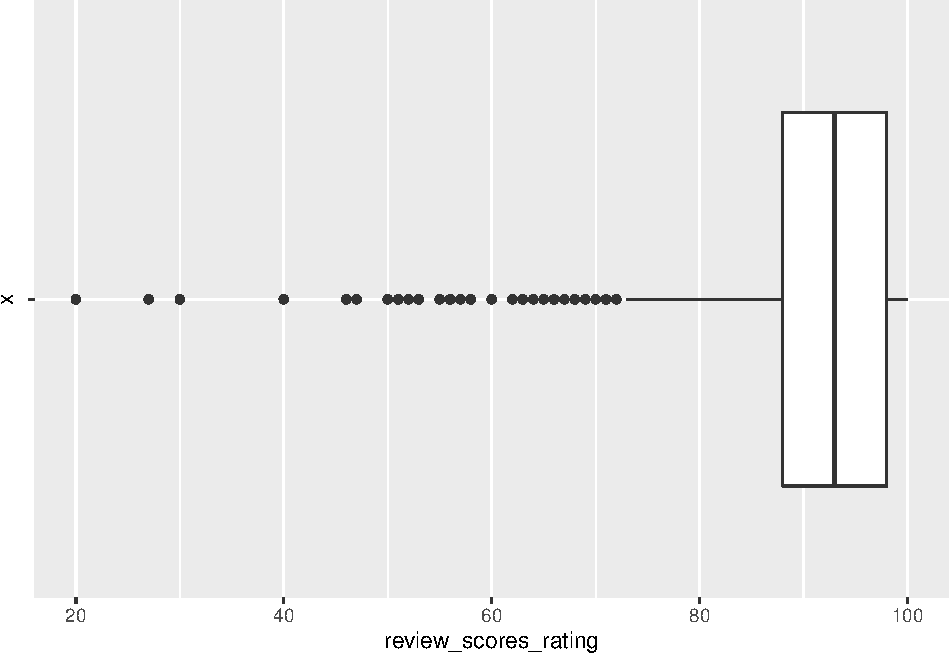
\includegraphics[width=0.5\linewidth]{anal_files/figure-latex/figures-side-43}

\begin{verbatim}
## [1] "Extended Summary Statistics"
##    Min. 1st Qu.  Median    Mean 3rd Qu.    Max.    NA's 
##   20.00   88.00   93.00   91.08   98.00  100.00    5971 
## [1] "sd:  10.4587403853611"
## [1] "vc:  0.114830482428774"
## [1] "variable  62 : review_scores_accuracy"
\end{verbatim}

\begin{verbatim}
## `stat_bin()` using `bins = 30`. Pick better value with `binwidth`.
\end{verbatim}

\begin{verbatim}
## Warning: Removed 5982 rows containing non-finite values (stat_bin).
\end{verbatim}

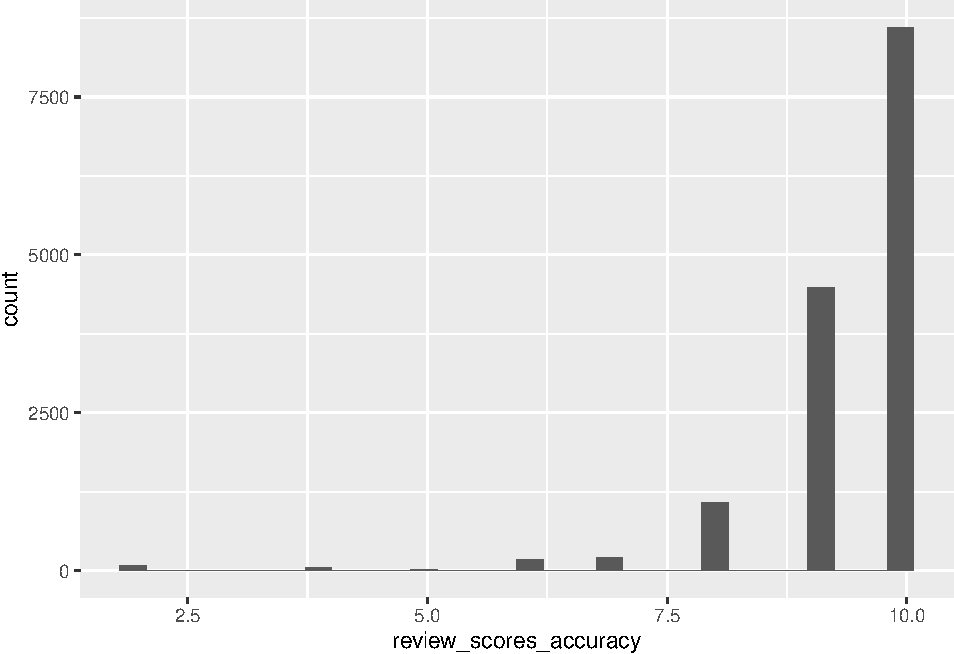
\includegraphics[width=0.5\linewidth]{anal_files/figure-latex/figures-side-44}

\begin{verbatim}
## Warning: Removed 5982 rows containing non-finite values (stat_boxplot).
\end{verbatim}

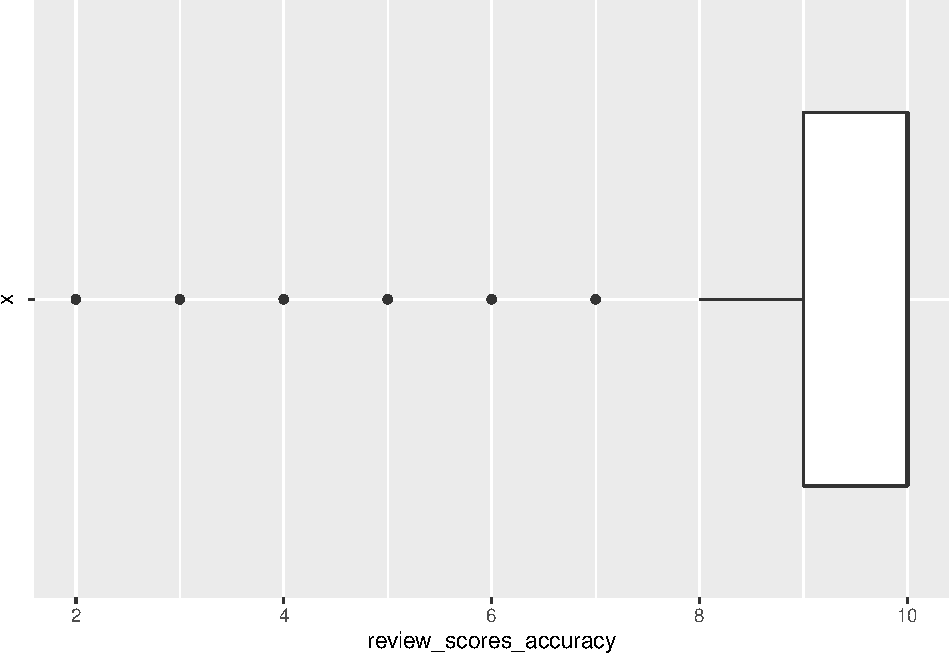
\includegraphics[width=0.5\linewidth]{anal_files/figure-latex/figures-side-45}

\begin{verbatim}
## [1] "Extended Summary Statistics"
##    Min. 1st Qu.  Median    Mean 3rd Qu.    Max.    NA's 
##   2.000   9.000  10.000   9.379  10.000  10.000    5982 
## [1] "sd:  1.04266849011004"
## [1] "vc:  0.111176384662649"
## [1] "variable  63 : review_scores_cleanliness"
\end{verbatim}

\begin{verbatim}
## `stat_bin()` using `bins = 30`. Pick better value with `binwidth`.
\end{verbatim}

\begin{verbatim}
## Warning: Removed 5980 rows containing non-finite values (stat_bin).
\end{verbatim}

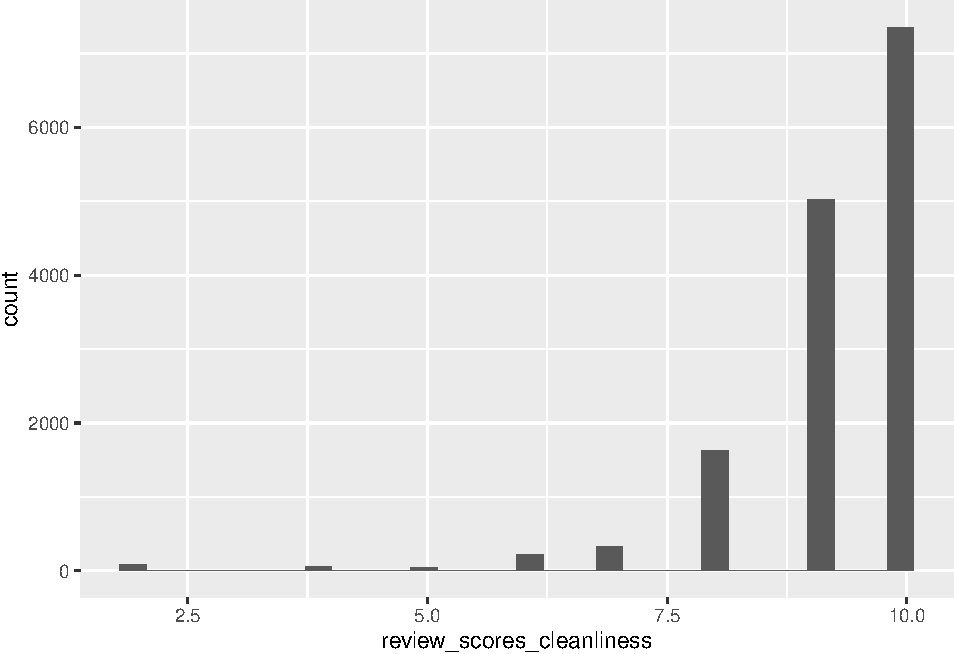
\includegraphics[width=0.5\linewidth]{anal_files/figure-latex/figures-side-46}

\begin{verbatim}
## Warning: Removed 5980 rows containing non-finite values (stat_boxplot).
\end{verbatim}

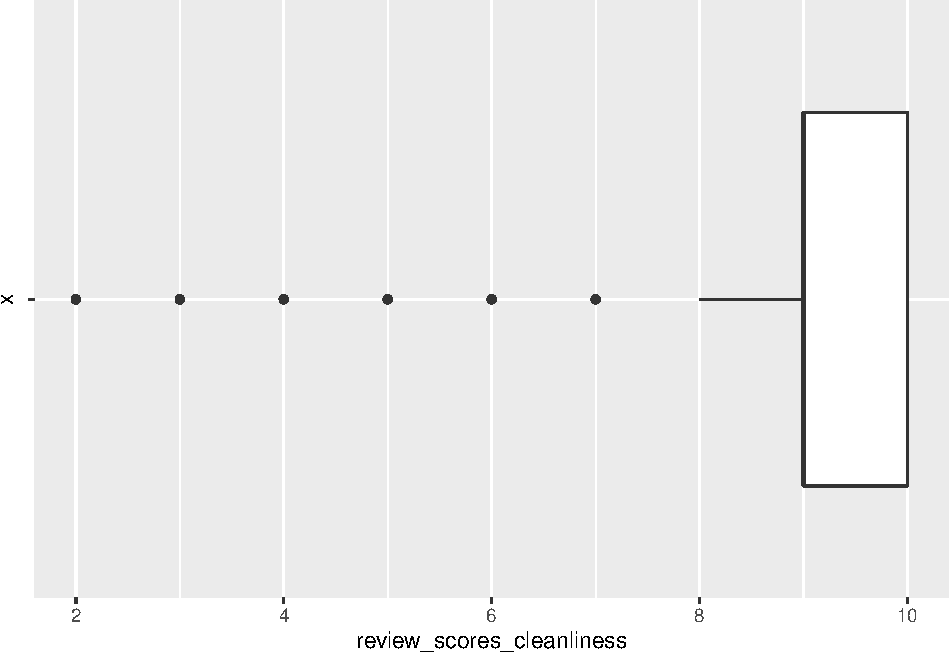
\includegraphics[width=0.5\linewidth]{anal_files/figure-latex/figures-side-47}

\begin{verbatim}
## [1] "Extended Summary Statistics"
##    Min. 1st Qu.  Median    Mean 3rd Qu.    Max.    NA's 
##   2.000   9.000   9.000   9.227  10.000  10.000    5980 
## [1] "sd:  1.10031287017275"
## [1] "vc:  0.119251994078246"
## [1] "variable  66 : review_scores_location"
\end{verbatim}

\begin{verbatim}
## `stat_bin()` using `bins = 30`. Pick better value with `binwidth`.
\end{verbatim}

\begin{verbatim}
## Warning: Removed 5985 rows containing non-finite values (stat_bin).
\end{verbatim}

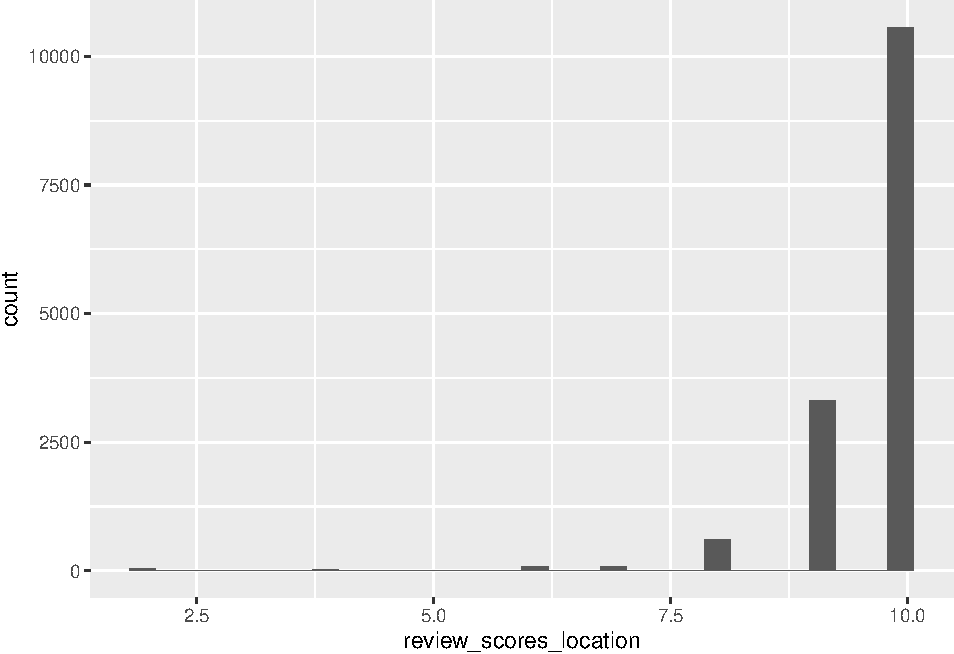
\includegraphics[width=0.5\linewidth]{anal_files/figure-latex/figures-side-48}

\begin{verbatim}
## Warning: Removed 5985 rows containing non-finite values (stat_boxplot).
\end{verbatim}

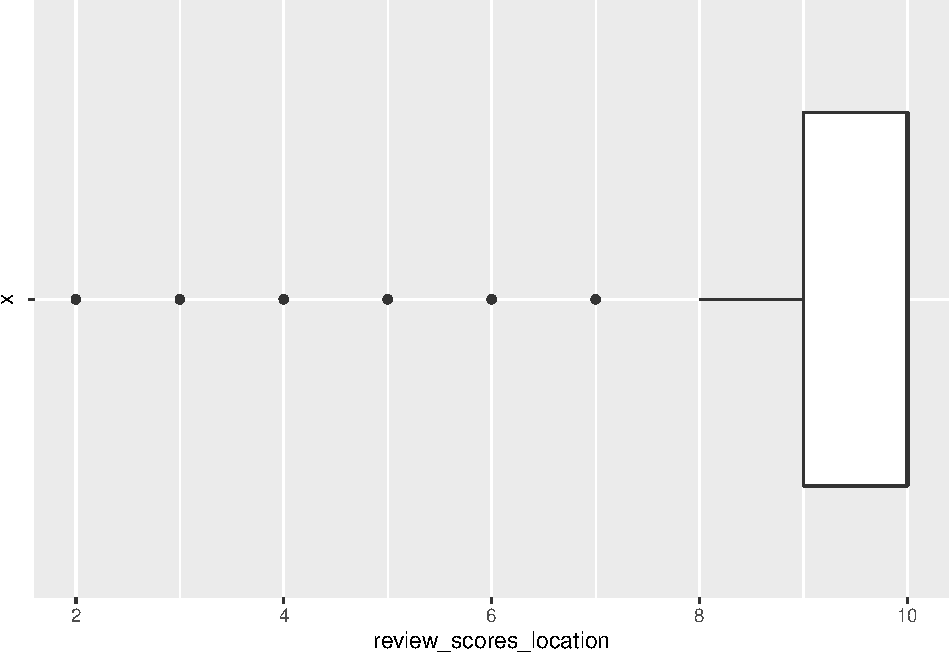
\includegraphics[width=0.5\linewidth]{anal_files/figure-latex/figures-side-49}

\begin{verbatim}
## [1] "Extended Summary Statistics"
##    Min. 1st Qu.  Median    Mean 3rd Qu.    Max.    NA's 
##   2.000   9.000  10.000   9.618  10.000  10.000    5985 
## [1] "sd:  0.788058627433689"
## [1] "vc:  0.0819339145567567"
## [1] "variable  67 : review_scores_value"
\end{verbatim}

\begin{verbatim}
## `stat_bin()` using `bins = 30`. Pick better value with `binwidth`.
\end{verbatim}

\begin{verbatim}
## Warning: Removed 5985 rows containing non-finite values (stat_bin).
\end{verbatim}

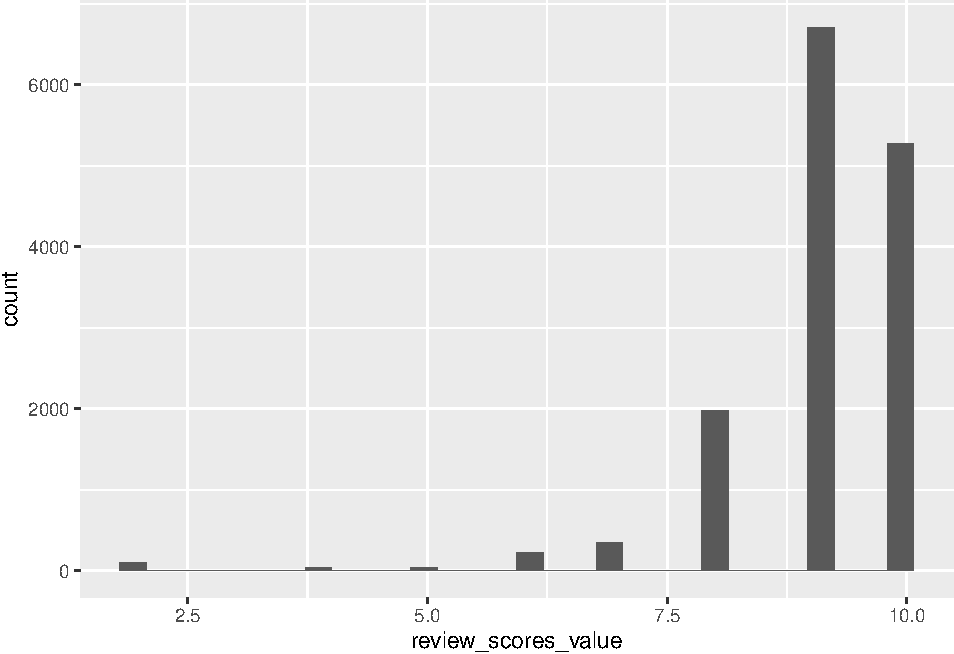
\includegraphics[width=0.5\linewidth]{anal_files/figure-latex/figures-side-50}

\begin{verbatim}
## Warning: Removed 5985 rows containing non-finite values (stat_boxplot).
\end{verbatim}

\includegraphics[width=0.5\linewidth]{anal_files/figure-latex/figures-side-51}

\begin{verbatim}
## [1] "Extended Summary Statistics"
##    Min. 1st Qu.  Median    Mean 3rd Qu.    Max.    NA's 
##   2.000   9.000   9.000   9.055  10.000  10.000    5985 
## [1] "sd:  1.0877510547065"
## [1] "vc:  0.120132968320041"
## [1] "variable  69 : instant_bookable"
\end{verbatim}

\includegraphics[width=0.5\linewidth]{anal_files/figure-latex/figures-side-52}
\includegraphics[width=0.5\linewidth]{anal_files/figure-latex/figures-side-53}

\begin{verbatim}
## [1] "Number of modalities:  2"
## [1] "Frequency table"
## 
## FALSE  TRUE 
##  9372 11331 
## [1] "Relative frequency table (proportions)"
## 
##    FALSE     TRUE 
## 0.452688 0.547312 
## [1] "Frequency table sorted"
## 
##  TRUE FALSE 
## 11331  9372 
## [1] "Relative frequency table (proportions) sorted"
## 
##     TRUE    FALSE 
## 0.547312 0.452688 
## [1] "variable  74 : reviews_per_month"
\end{verbatim}

\begin{verbatim}
## `stat_bin()` using `bins = 30`. Pick better value with `binwidth`.
\end{verbatim}

\begin{verbatim}
## Warning: Removed 5731 rows containing non-finite values (stat_bin).
\end{verbatim}

\includegraphics[width=0.5\linewidth]{anal_files/figure-latex/figures-side-54}

\begin{verbatim}
## Warning: Removed 5731 rows containing non-finite values (stat_boxplot).
\end{verbatim}

\includegraphics[width=0.5\linewidth]{anal_files/figure-latex/figures-side-55}

\begin{verbatim}
## [1] "Extended Summary Statistics"
##    Min. 1st Qu.  Median    Mean 3rd Qu.    Max.    NA's 
##   0.010   0.210   0.710   1.179   1.770  21.410    5731 
## [1] "sd:  1.28741924372801"
## [1] "vc:  1.09231185933215"
## [1] "variable  77 : host_since_season"
\end{verbatim}

\includegraphics[width=0.5\linewidth]{anal_files/figure-latex/figures-side-56}
\includegraphics[width=0.5\linewidth]{anal_files/figure-latex/figures-side-57}

\begin{verbatim}
## [1] "Number of modalities:  5"
## [1] "Frequency table"
## 
## Winter Spring Summer Autumn   <NA> 
##   4988   5411   5251   5031     22 
## [1] "Relative frequency table (proportions)"
## 
##      Winter      Spring      Summer      Autumn        <NA> 
## 0.240931266 0.261363087 0.253634739 0.243008260 0.001062648 
## [1] "Frequency table sorted"
## 
## Spring Summer Autumn Winter   <NA> 
##   5411   5251   5031   4988     22 
## [1] "Relative frequency table (proportions) sorted"
## 
##      Spring      Summer      Autumn      Winter        <NA> 
## 0.261363087 0.253634739 0.243008260 0.240931266 0.001062648 
## [1] "variable  75 : host_since_year"
\end{verbatim}

\includegraphics[width=0.5\linewidth]{anal_files/figure-latex/figures-side-58}
\includegraphics[width=0.5\linewidth]{anal_files/figure-latex/figures-side-59}

\begin{verbatim}
## [1] "Number of modalities:  14"
## [1] "Frequency table"
## 
## 2008 2009 2010 2011 2012 2013 2014 2015 2016 2017 2018 2019 2020 <NA> 
##    1   28  249 1179 1988 2395 1794 2392 2101 2126 2249 2973 1220    8 
## [1] "Relative frequency table (proportions)"
## 
##         2008         2009         2010         2011         2012         2013 
## 4.830218e-05 1.352461e-03 1.202724e-02 5.694827e-02 9.602473e-02 1.156837e-01 
##         2014         2015         2016         2017         2018         2019 
## 8.665411e-02 1.155388e-01 1.014829e-01 1.026904e-01 1.086316e-01 1.436024e-01 
##         2020         <NA> 
## 5.892866e-02 3.864174e-04 
## [1] "Frequency table sorted"
## 
## 2019 2013 2015 2018 2017 2016 2012 2014 2020 2011 2010 2009 <NA> 2008 
## 2973 2395 2392 2249 2126 2101 1988 1794 1220 1179  249   28    8    1 
## [1] "Relative frequency table (proportions) sorted"
## 
##         2019         2013         2015         2018         2017         2016 
## 1.436024e-01 1.156837e-01 1.155388e-01 1.086316e-01 1.026904e-01 1.014829e-01 
##         2012         2014         2020         2011         2010         2009 
## 9.602473e-02 8.665411e-02 5.892866e-02 5.694827e-02 1.202724e-02 1.352461e-03 
##         <NA>         2008 
## 3.864174e-04 4.830218e-05 
## [1] "variable  78 : host_response_rate_cat"
\end{verbatim}

\includegraphics[width=0.5\linewidth]{anal_files/figure-latex/figures-side-60}
\includegraphics[width=0.5\linewidth]{anal_files/figure-latex/figures-side-61}

\begin{verbatim}
## [1] "Number of modalities:  6"
## [1] "Frequency table"
## 
##  very low       low   average      high very high      <NA> 
##       588       240       487       996     11218      7174 
## [1] "Relative frequency table (proportions)"
## 
##   very low        low    average       high  very high       <NA> 
## 0.02840168 0.01159252 0.02352316 0.04810897 0.54185384 0.34651983 
## [1] "Frequency table sorted"
## 
## very high      <NA>      high  very low   average       low 
##     11218      7174       996       588       487       240 
## [1] "Relative frequency table (proportions) sorted"
## 
##  very high       <NA>       high   very low    average        low 
## 0.54185384 0.34651983 0.04810897 0.02840168 0.02352316 0.01159252 
## [1] "variable  79 : host_acceptance_rate_cat"
\end{verbatim}

\includegraphics[width=0.5\linewidth]{anal_files/figure-latex/figures-side-62}
\includegraphics[width=0.5\linewidth]{anal_files/figure-latex/figures-side-63}

\begin{verbatim}
## [1] "Number of modalities:  6"
## [1] "Frequency table"
## 
##  very low       low   average      high very high      <NA> 
##       852       379       713      1584     13737      3438 
## [1] "Relative frequency table (proportions)"
## 
##   very low        low    average       high  very high       <NA> 
## 0.04115346 0.01830653 0.03443945 0.07651065 0.66352703 0.16606289 
## [1] "Frequency table sorted"
## 
## very high      <NA>      high  very low   average       low 
##     13737      3438      1584       852       713       379 
## [1] "Relative frequency table (proportions) sorted"
## 
##  very high       <NA>       high   very low    average        low 
## 0.66352703 0.16606289 0.07651065 0.04115346 0.03443945 0.01830653
\end{verbatim}
